% August 2017 (TOC contents linked in blue in pdf file)
%This template was prepared by Dorothea F. Brosius of the
%Institute for Electronics and Applied Physics, University of Maryland, College Park, MD
%The template was last updated in August 2017
%Thesis Main Page used with thesis.sty based on the
%University of Maryland Electronic Thesis and Dissertation (ETD) Style Guide (2016)

%The YourInformation file was created by Freja Nordsiek, 2014.
%Code for linking the TOC titles to the text in the pdf file was created by Freja Nordsiek, 2014.

% Select the version that fits how you are making this LaTeX document (its driver).
% The first two are the most likely ones to be needed.

 \newcommand{\mydriver}{pdflatex} %Making a PDF directly using pdflatex.
%\newcommand{\mydriver}{dvipdfmx} %Making a DVI and converting that to PDF using dvipdfmx.
%\newcommand{\mydriver}{dvipdfm} %Making a DVI and converting that to PDF using dvipdfm.
%\newcommand{\mydriver}{dvips} %Making a DVI and converting that to PS using dvips (may later be converted to PDF).
%\newcommand{\mydriver}{dvipsone} %Making a DVI and converting that to PS using dvipsone (may later be converted to PDF).
%\newcommand{\mydriver}{ps2pdf} %Same as the one for dvips except it is compatible with Ghostscript's PDF writer.


\documentclass[12pt,\mydriver]{thesis}  %12pt is larger than 11pt

\usepackage{titlesec}
   \titleformat{\chapter}
      {\normalfont\large}{Chapter \thechapter:}{1em}{}
\usepackage{graphicx}
\usepackage{cite}
\usepackage{lscape}
\usepackage{indentfirst}
\usepackage{latexsym}
\usepackage{multirow}
\usepackage{epstopdf}
\usepackage{tabls}
\usepackage{wrapfig}
\usepackage{slashbox}
\usepackage{longtable}
\usepackage{supertabular}
\usepackage{subeqn}
\usepackage{subfigure}

%hyperref
\usepackage[colorlinks=true,urlcolor=black,linkcolor=blue,citecolor=blue]{hyperref}

\newcommand{\tbsp}{\rule{0pt}{18pt}} %used to get a vertical distance after \hline
\renewcommand{\baselinestretch}{2}
\setlength{\textwidth}{5.9in}
\setlength{\textheight}{9in}
\setlength{\topmargin}{-.50in}
%\setlength{\topmargin}{0in}    %use this setting if the printer makes the the top margin 1/2 inch instead of 1 inch
\setlength{\oddsidemargin}{.55in}
\setlength{\parindent}{.4in}
\pagestyle{empty}

\begin{document}
\pagestyle{empty}
\begin{abstract}
	There are two kinds of type disciplines of different natures:
	On the one hand, we know that statically typed languages are reliable and efficient,
	but it is not very convenient when it comes to program prototyping or refactoring.
	On the other hand, dynamically typed languages does not prevent programs from execution
	through ahead-of-time checks, which makes them flexible but at the same time
	mistakes become harder to spot and programs more difficult to maintain over time.
	
	It is only natural that we look into
	integrating static and dynamic type systems.
	Among one of the related lines of research is gradual typing, which
	intends to support not just fully static and full dynamic type systems
	but also those partially typed programs.
	By providing control over which part of the program should be checked
	by the type system, programmers are free to evolve programs
	towards either static or dynamic typing in a smooth and consistent manner.

	Despite that gradual type systems are well-studied research topics,
	extending existing languages to support them is far from trivial task:
	to make a successful gradual typing extension,
	the type system is needed to be extended, types to be designed,
	extra features to be introduced and tradeoff to be made, all of which
	require taking into account the design, programming idiom and user community that
	the original language has.
	In this survey, we will walk through the relevant research literature on extending
	existing languages to support gradual types,
	discuss challenges and solutions about making these extensions,
	and look into related works and the future of gradual typing.

\end{abstract} %(must be first, required, non-numbered)
%Titlepage

\thispagestyle{empty}
\hbox{\ }
\vspace{1in}
\renewcommand{\baselinestretch}{1}
\small\normalsize
\begin{center}

\large{{TITLE1 \\
TITLE2}}\\
\ \\
\ \\
\large{by} \\
\ \\
\large{Fang Cheng}%Your full name as it appears in University records.
\ \\
\ \\
\ \\
\ \\
\normalsize
Dissertation submitted to the Faculty of the Graduate School of the \\
University of Maryland, College Park in partial fulfillment \\
of the requirements for the degree of \\
Master of Science \\
2018
\end{center}

\vspace{7.5em}

\noindent Advisory Committee: \\
Professor Rajarshi Roy, Chair/Advisor \\
Dr. Parvez N. Guzdar, Co-Advisor \\
Professor Robert W. Gammon \\
Professor Thomas Antonsen \\
Professor Edward Ott
 %(must follow Abstract, required, non-numbered)
%Copyright

\thispagestyle{empty}
\hbox{\ }

\vfill
\renewcommand{\baselinestretch}{1}
\small\normalsize

\vspace{-.65in}

\begin{center}
\large{\copyright \hbox{ }Copyright by\\
Bhaskar Khubchandani  %Type your name as it appears in University records
\\
2004}
\end{center}

\vfill

\newpage

\hbox{\ }
\newpage
 %(highly recommended, non-numbered)

%Pages from this point start at lower-case Roman number ii)
\pagestyle{plain} \pagenumbering{roman} \setcounter{page}{2}
\addcontentsline{toc}{chapter}{Preface}
%Preface
\pagestyle{plain}\pagenumbering{roman} \setcounter{page}{2}
\renewcommand{\baselinestretch}{2}
\small\normalsize
\hbox{\ }

\vspace{-.65in}

\begin{center}
\large{Preface}
\end{center}


If needed.
  %(if present, start at lower-case Roman number ii)
\addcontentsline{toc}{chapter}{Foreword}
%Foreword

\renewcommand{\baselinestretch}{2}
\small\normalsize
\hbox{\ }
 
\vspace{-.65in}

\begin{center}
\large{Foreword} 
\end{center} 

If needed.
 %(if present, lower-case Roman)
\addcontentsline{toc}{chapter}{Dedication}
%Dedication

\renewcommand{\baselinestretch}{2}
\small\normalsize
\hbox{\ }
 
\vspace{-.65in}

\begin{center}
\large{Dedication}
\end{center} 

If needed.
 %(if present, lower-case Roman)
\addcontentsline{toc}{chapter}{Acknowledgements}
%Acknowledgments

\renewcommand{\baselinestretch}{2}
\small\normalsize
\hbox{\ }
 
\vspace{-.65in}

\begin{center}
\large{Acknowledgments} 
\end{center} 

\vspace{1ex}

I owe my gratitude to all the people who have made this thesis possible and because of whom my graduate experience has been one that I will cherish forever.

First and foremost I'd like to thank my advisor, Professor Rajarshi Roy for giving me an invaluable opportunity to work on challenging and extremely interesting projects over the past four years. He has always made himself available for help and advice and there has never been an occasion when I've knocked on his door and he hasn't given me time. It has been a pleasure to work with and learn from such an extraordinary individual.

I would also like to thank my co-advisor, Dr. Parvez Guzdar. Without his extraordinary theoretical ideas and computational expertise, this thesis would have been a distant dream. Thanks are due to Professor Robert Gammon, Professor Edward Ott and Professor Thomas Antonsen for agreeing to serve on my thesis committee and for sparing their invaluable time reviewing the manuscript.

My colleagues at the nonlinear optics laboratory have enriched my graduate life in many ways and deserve a special mention. David DeShazer helped me start-off by rewriting the basic simulation code in a user-friendly format. Christian Silva provided help by setting up the GRENOUILLE apparatus and performing some of the simulations. My interaction with  Rohit Tripathi, Ryan McAllister, Vasily Dronov, Min-Young Kim, Elizabeth Rogers, William Ray, Jordi Garcia Ojalvo, Riccardo Meucci, Atsushi Uchida, and Fabian Rogister has been very fruitful. I'd also like to thank Wing-Shun Lam and Benjamin Zeff for providing the LaTex style files for writing this thesis.

I would also like to acknowledge help and support from some of the staff members. Donald Martin's technical help is highly appreciated, as is the computer hardware support from Edward Condon, LaTex and software help from Dorothea Brosius and purchasing help from Nancy Boone.

I owe my deepest thanks to my family - my mother and father who have always stood by me and guided me through my career, and have pulled me through against impossible odds at times. Words cannot express the gratitude I owe them. I would also like to thank Dr. Mohan Advani, Dr. Vasudeo Paralikar and Dr. Vinod Chaugule who are like family members to me.

My housemates at my place of residence have been a crucial factor in my finishing smoothly. I'd like to express my gratitude to Sivasankar Pandeti, Jayakumar Patil, Amit Trehan and Punyaslok Purakayastha for their friendship and support.

I would like to acknowledge financial support from the Office of Naval Research (ONR), Physics, for all the projects discussed herein.

It is impossible to remember all, and I apologize to those I've inadvertently left out.

Lastly, thank you all and thank God!
 %(if present, lower-case Roman)

\renewcommand{\baselinestretch}{1}
\small\normalsize
\tableofcontents %(required, lower-case Roman)
\newpage
\listoftables %(if present, lower-case Roman)
\newpage
\listoffigures %(if present, lower-case Roman)
\newpage
% LIST OF ABBREVIATIONS
\addcontentsline{toc}{chapter}{List of Abbreviations}
%List of Abbreviations


\renewcommand{\baselinestretch}{1}
\small\normalsize
\hbox{\ }

\vspace{-4em}

\begin{center}
\large{List of Abbreviations}
\end{center} 

\vspace{3pt}

\begin{supertabular}{ll}
AAA & Antiaircraft artillery \\
ABCCC & Airborne Battlefield Command and Control Center \\
AEHF & Advanced Extremely High Frequency \\
AGM & Air-to-ground guided missile \\
AIT & Assembly, Integration, and Testing \\
AOR & Area of Responsibility \\
APAM & Anti-personnel, anti-material \\
ASOC & Air Support Operations Center \\
ATACM & Army Tactical Missile System \\
ATO & Air Tasking Order \\
AWACS & Airborne Warning and Control System \\
\\
BAT & Brilliant Ani-Armor Submunition \\
BDA & Bomb-damage assessment  \\
BFT & Blue Force Tracking \\
BLOS & Beyond Line-of-Sight \\
BMD & Ballistic Missile Defense \\
\\
C$^{3}$ & Command, Control, and Communications \\
CAFMS & Computer-aided Force Management System \\
CALCM & Conventional Air-Launched Cruise Missile \\
CBU & Cluster Bomb Unit \\
CCAFS & Cape Canaveral Air Force Station \\
CENTAF & CENTCOM's Air Force component \\
CENTCOM & U.S. Central Command \\
CINC & Commander-in-Chief \\
CONUS & Continental United States \\
\\
DAGR & Defense Advanced GPS Reciever \\
DMA & Defense Mapping Agency \\
DOD & Department of Defense \\
DOP & Dilution of Precision \\
DOT & Department of Transportation \\
DSMAC & Digital Scene Mapping Area Correlator \\
\\
EFOG-M & Enhanced Fiber Optic Guided Missile \\
\\
FAA & Federal Aviation Administration \\
FLIR & Forward-looking infrared \\
\\
GAM & Global Positioning System Aided Munition \\
GPS & Global Positioning System \\
GWAPS & Gulf War Air Power Survey \\
\\
HARM & High-Speed Antiradiation Missile \\
HEO & Highly Elliptical Orbit \\
\\
IADS & Integrated Air Defense System \\
ICBM & Inter-Continental Ballistic Missile \\
INS & Inertial navigation system \\
IIR & Imaging infrared \\
IR & Infrared \\
ISR & Intelligence, Surveillance, and Reconnaissance \\
\\
JDAM & Joint Direct Attack Munition \\
JFC & Joint Force Commander \\
JSOW & Joint Standoff Weapon \\
\\
LANTIRN & Low-Altitude Navigation and Targeting Infrared for Night System \\
LEO & Low Earth Orbit \\
LGB & Laser-guided bomb \\
\\
MAJIC & Microsatellte Area-Wide Joint Information Communication \\
MARCENT & CENTCOM's Marine component \\
MARS & Mid-Atlantic Regional Spaceport \\
MLRS & Multiple Launch Rocket System \\
MUOS & Mobile User Objective System \\
\\
NASA & National Aeronautics and Space Administration \\
NAVCENT & CENTCOM's Navy component \\
NPOESS & National Polar-Orbiting Operational Environmental Satellite System \\
\\
ORS & Opertionally Responsive Space \\
ORSO & Operationally Responsive Space Office \\
\\
PDOP & Position Dilution of Precision \\
PGM & Precision-guided munition \\
P$^{3}I$ & Preplanned Product Improvement \\
PnP & Plug and Play \\
PnPSat & Plug and Play Satellite \\
PPS & Precise Positioning Service \\
\\
RCS & Radar cross section \\
\\
SA & Situational Awareness \\
SADARM & Sense and Destroy Armor Munition \\
SAM & Surface-to-air missile \\
SAR & Synthetic aperture radar \\
SBIRS & Space Based Infrared System \\
SEAD & Suppression of enemy air defenses \\
SFW & Sensor Fuzed Weapon \\
SIGINT & Signal Intelligence \\
SLAM & Standoff Land Attack Missile \\
SLAM-ER & SLAM-Expanded Response \\
SpaceX & Space Exploration Technologies Corporation \\
SPS & Standard Positioning Service \\
\\
TACC & Tactical Air Control Center \\
TACS & Tactical Air Control System \\
TACP & Tactical Air Control Party \\
TASM & Tomahawk Anti-Ship Missile \\
TBIP & Tomahawk Baseline Improvement Program \\
TERCOM & Terrain Contour Mapping \\
TFR & Terrain-following radar \\
TLAM & Tomahawk Land Attack Missile \\
\\
USAF & U.S. Air Force \\
\\
VAFB & Vandenberg Air Force Base \\
\\
WGS & Wideband Global SATCOM \\
%$\alpha$ & alpha \\
%$\beta$  & beta \\
%&  \\ 
%IREAP & Institute for Research in Electronics and Applied Physics \\
%NSA & National Security Agency
\end{supertabular}


\newpage
\setlength{\parskip}{0em}
\renewcommand{\baselinestretch}{2}
\small\normalsize

%Pages from this point start at Arabic numeral 1
\setcounter{page}{1}
\pagenumbering{arabic}
%Chapter 1

% \renewcommand{\thechapter}{1}

\section{Introduction}

% TODO: about detect and localize error

Type system defines sets of rules about programs, which can be checked by a machine
in a systematic way.
One can assign types to appropriate language concepts like
variables, functions and classes to describe expected behaviors
and how they interact with each other.
Then type system takes the responsibility of ensuring that types are respected and
type errors prevent erroneous part of a program from execution.

There are other benefits of type systems besides automated checking:
types can be used to reveal optimization opportunities,
can serve as simple documentation to programmers or
provide hints to development tools to automate navigation, documentation lookup
or auto-completion.

All these benefits make type system an important part of programming languages,
and there are different ways of accommodating languages with type systems.
The most noticeable difference is the process of checking programs again type rules,
which is also known as type checking.
It occurs either statically ahead of program execution, or dynamically at runtime.
For a static type system, ill-typed programs are rejected by compiler and
no executable can be produced until all type errors are fixed.
For a dynamic type system, type information is examined at runtime and type errors result
in abortion of the program or exceptions being raised
instead of causing segmentation faults or other worse consequences.
Static and dynamic type system both have their advantages and disadvantages,
and languages make different choices depending on their needs.

In this chapter, we start off by discussing static and dynamic type systems,
which motivates research works that attempted to combine both within one system
in order to take the benefits from the two,
which in return gives birth to many possible solutions.
One particular example among them is gradual typing.

\subsection{Strengths and Weaknesses of Static and Dynamic Typing}

The difference between static and dynamic typing is the difference
between whether type checking occurs ahead of execution or at runtime.
This section discusses advantages and disadvantages of both.

\newcommand{\tnum}{\textbf{num}}
\newcommand{\tstr}{\textbf{str}}
\newcommand{\tbool}{\textbf{bool}}
\newcommand{\tarr}[2]{#1 \rightarrow #2}

In this section we use $\tau_0, \tau_1, \ldots$ for type variables.
$\tbool$, $\tnum$ and $\tstr$ are types of
boolean values, numbers and strings respectively.\
Tuple types are notated as $(\tau_0, \tau_1, \ldots)$,
and the type notation for functions that takes as input a value of type $\tau_0$
and returns a value of $\tau_1$ is $\tarr{\tau_0}{\tau_1}$.
We use $o : \tau$ to mean that a term $o$ is assigned type $\tau$.
For example $f : \tarr{(\tnum, \tnum)}{\tnum}$ is a function that
takes a tuple of two numbers as input and returns a number.

\subsubsection{Static Type Systems}

%TODO: type system or language?

A static type system is preferred if robustness and performance
is the main goal of a language.
Because type checking occurs ahead of execution,
ill-typed programs are rejected before it can start, and
when a program typechecks,
one can therefore expect no type error to occur and
no extra cost is paid for typechecking at runtime.

For a static type system to work, all variables, functions, etc. in a program
will need to be assigned types. This is usually done by programmers or through the
means of type inference, which is a technique that infers types using
available type information. This is both an advantage and a disadvantage
of a static type system: having type annotations improves readability
and since programmers are required to keep the consistency between type and code,
type also serves as simple, faithful documentation. But on the other hand,
adding and maintaining type annotations can also considered a burden.

Having static known type information also helps in terms of performance in other ways.
For example, In many programming languages, arithmetic functions are polymorphic.
It is allowed for \textbf{a} and \textbf{b} to have different numeric types in \textbf{a + b}, a cast will be inserted to ensure arithmetic primitives only deals with addition of compatible types: if we are adding integer \textbf{b} to a floating number \textbf{a}, then \textbf{b} will be casted so we can call addition primitive that expected floating numbers on both sides.
A dynamic language would have to figure out types of \textbf{a} and \textbf{b} at runtime, make decision about whether casting is required or which primitive addition to call all at runtime. But with type information statically available,
these decisions can be made ahead of execution,
resulting in improved performance at runtime.

Besides extra effort of maintaining type annotations,
the disadvantage of a statically type language often lies in the lack of runtime flexibility.
If we want to write a program that deals with data whose structure is
unknown at compile time, runtime inspection must be possible.
While typical dynamically typed languages allow inspect of types or object properties,
some extra work are required for a statically typed language
to keep type information available at runtime.

In addition, it is often less convenient for programmers to prototype
in statically typed languages: it involves trial and error to find the best implementation
to solve a problem, which means the ability to write partial programs,
make frequent changes to structure of variables and functions, but these features are not easily available for a statically typed language.

\subsubsection{Dynamic Type Systems}

Dynamic type systems do typechecking at runtime, which is best suited for
languages designed for scripting and fast prototyping.
A shell script, for example, runs other executables and feeds one's output to another, effectively gluing programs together.
In such a case, we have little to no knowledge about these executables ahead of time,
making statically type checking impractical.
And when it comes to prototyping,
it is more important for programmers to execute the code and make modifications accordingly
than to enforce correctness and consistency through whole program.
In such scenario, it is more convenient to delay type checking until
it is required at runtime.

However, it is also easy to spot weaknesses of dynamic type systems.
Despite that type checking does not happen ahead of execution,
programmers usually have facts about behaviors of programs,
which is often described in comments or through naming of variables and functions without a systematic way of verifying them.
As program develops, it is easy to make changes and forget updating these descriptions accordingly, which forces future maintainers to go back and rediscover these facts, causing maintenance difficulties.

%TODO: throw error at runtime

Furthermore, without type information statically available,
dynamic type system needs to maintain runtime information
and rely on it to implement expected semantics.
For example, if it is allowed for a language to condition on non-boolean values,
its type has to be available at runtime in order to
determine how to cast it into a boolean value at runtime.

Optimization could also be hindered for a dynamically type language: 
array cloning can be implemented efficiently as memory copy instructions knowing the array in question contains only primitive values but no reference or pointers, whereas without prior knowledge like this, every element of the array has to be traversed and even recursively cloned.


\subsection{Combining the benefits of the two}

%TODO could have more to say.

One might have noticed that
while static type checking happens ahead of execution,
dynamic one is performed at runtime.
Therefore they are not fundamentally mutually exclusive to each other.

Indeed, researchers have been looking at different angles of
the possibility of integrating both type discipline within one.
several attempts are motivated to put these two type systems in one.
In this section, we will discuss about these research works.

\subsubsection{Design Goals}

Summarizing pros and cons of static and dynamic typed languages,
we now have a picture of an ideal type system, it should have following features:

\begin{itemize}
	\item \textbf{Detect and rule out errors ahead of program execution.}
	This is one main purpose of having a static type system. When a program starts running,
	type errors should already be eliminated and runtime overhead should be minimized
	to keep its performance close to that of a static type system.
	\item \textbf{Delay typechecking until needed at runtime.}
	This is the crucial feature of a dynamic type system,
	it allows ill-typed or partially written programs to execute,
	which makes it suitable in situations where static type information
	is limited or fast prototyping is preferred over robustness or runtime performance.
\end{itemize}

Aside from these two goals, type annotations can also be used for
other purposes like optimization and providing hints to development tools.
For a language with this new type system, it should also be possible.

\subsubsection{A Introduction to Gradual Typing}

\newcommand{\dyn}{\textbf{dyn}}

Gradual typing is one possible approach that meets our design goal.
It captures the fact that type information might only be partially known
ahead of execution by introducing a special type that indicates partial types.
It attempts to typecheck programs like a static type system does, but delays
typechecking on partial types until sufficient type information is available
at runtime.

In the following sections, we will introduce it
as an extension to static type system.
But it is also possible and practical to support gradual typing by
extending a dynamic type system.

% TODO: in fact maj of langs are extended from dynamic ones

\paragraph{Dynamic Type and Type Consistency}

Gradual type system introduces a special type on top of a static type system
to capture the idea that type information might only be partially known
ahead of execution.
The special type is usually called a ``dynamic type'', we introduce a special type $\dyn$ for it.

To deal with dynamic types, type consistency is introduced
to accommodate type judgments for gradual typing.
Figure ? shows rules for type consistency relation.

\begin{math}
\inferrule*[left=(CREFL)]{ }{\tau \sim \tau}
\inferrule*[left=(CFUNC)]
  {\sigma_1 \sim \tau_1 \\ \sigma_2 \sim \tau_2}
  {\tarr{\sigma_1}{\sigma_2} \sim \tarr{\tau_1}{\tau_2} }
\end{math}

\begin{math}
\inferrule*[left=(CUNR)]{ }{\tau \sim \dyn}
\inferrule*[left=(CUNL)]{ }{\dyn \sim \tau}
\end{math}

In general, two types are consistent when
their type structures do not conflict with each other.
For example, $\tbool$ is consistent with type $\dyn$
despite that the latter is less precise;
$\tarr{\tnum}{\dyn}$ is consistent with both $\tarr{\dyn}{\tnum}$ and $\tarr{\dyn}{\dyn}$,
because all these types are functions that accepts one value and returns another and
$\tnum$ and $\dyn$ are consistent with each other.
However $\tarr{\dyn}{\dyn}$ is never consistent with $\tbool$,
because the former is a function type while the latter a boolean value,
whose type structures do not match.

In order to perform static typechecking, it is required that
all terms in the program to must have types ahead of execution.
In a gradual type system, this is no longer required:
for a specific term,
if programmers choose not to give a type annotation, it will be assigned type $\dyn$.
This still allows static typechecking to detect errors because
for types that contains $\dyn$, it is not totally ignored, but checked
up to the point where the structure of type is known.

On the other hand, a dynamically type program can now be statically typechecked
by considering it to be a program without any type annotation.
This is still beneficial, as some literal values and primitives will still have their built-in types,
an obvious misuse like taking the square root of a string value can now be detected ahead of execution
instead of raising runtime exceptions.

\paragraph{Cast Insertion and Runtime Typechecking}

As we can see gradual type system attempts to contain both statically and dynamically typed programs.
However, because of presence of dynamic types,
the type system cannot be sound by only have static typechecking.
Imagine function $f : \tarr{\tnum}{\dyn}$ and variable $v : \dyn$, while the function application
$f v$ can pass static typechecking, the runtime value of $t$ might turn out to be a string
and now the application is ill-typed.

The problem lies in the fact that some terms might be assigned with types that contains
$\dyn$, its runtime counterpart are precise, which is not checked during static typechecking.
To solve this problem, casts are inserted at appropriate locations, which then
allows type errors to be detected at runtime.
Suppose we have a cast function $c : \tarr{\dyn}{\tnum}$, function application $f v$
then becomes $f (c v)$, which still typechecks, but whenever we need to pass a runtime value to $f$,
its runtime is always checked by $c$ to decide whether to pass the value to $f$ or raise
a type error.
%TODO: from Gradual Typing for Functional Languages

\paragraph{Optional Type Annotation and ``pay-as-you-go''}

So far we have seen that gradual type system introduces a dynamic type,
which allows accepting both statically and dynamically typed programs during static typechecking.
But what is more important is that it creates a middle ground in which programs
can be partially annotated with types:
in a gradual type system, terms are either explicitly given a type,
or, when type annotation is missing, given $\dyn$ type.
This renders all type annotations to be optional and allows programmers
to have more control over what they need from typechecking:
for an originally statically typed program, we can now write terms without giving a type,
this allows easy prototyping; for an originally dynamically typed program,
some parts of it might already been stable and robust enough, annotating these parts
with type allows some effort of ensuring correctness being shifted to typechecking.

For example, one might wish to implement a function $f$ that expects a string value
as input. There are two approaches: we can either give $f$ a type annotation:
$f : \tarr{\textbf{str}}{\dyn}$. By doing so, type system takes the responsibility
of making sure that the input type is indeed a string. Alternatively,
we can inspect type of the input value at runtime ourselves.
A static type system allows us to do the former, but a return type must either
be given explicitly or inferred. And a dynamic type system does the later, but
we cannot statically detect any mistake like applying a number literal to $f$.
However, a gradual type system finds the balance between two,
it allows us to give input value a type without worrying about
giving a return type if not needed,
therefore programmer only pays for what they want from a type system.

%TODO more to say



\paragraph{Gradual Guarantee}

Regarding the term gradual typing itself,
Siek, Vitousek, Cimini and Boyland's work gives a detailed explanation of
the original intention.
Several works we are going to discuss in the following few chapters respects
such idea:

\begin{itemize}
	\item \textbf{Gradual typing includes both fully static and fully dynamic}
	A gradually typed language should be a superset of both a statically typed
	language and a dynamically typed one.
	Except for cases of type errors, evaluating a fully type-annotated program
	should have the same result as its untyped counterpart.
	\item \textbf{Gradual typing provides sound interoperability}
	\item \textbf{Gradual typing enables gradual evolution}
\end{itemize}


\subsubsection{Alternatives}

There are other type systems that bring benefits of the two together.
Cartwright and Fagan's introduced soft typing, which is a type system
that programers do not write type annotations but use type inference to
assign appropriate types to terms, and runtime checks are inserted as needed.
The drawback of this design is that programmers do not have control over types.
%TODO probably more drawbacks
Quasi-static typing is another attempt, with the idea of dynamic type in use,
it chooses to use a subtyping relation and allows both up-casts and down-casts.
A second pass of plausibility checking detects incompatible casts and signals the program
in question as ill-typed. However its typechecking algorithm did not receive a correct proof,
and it does not statically catch all type errors (TODO: ref)
in the process of attempting the proof, Siek and Taha finds a better solution, 
which results in gradual typing that we have seen today.
%TODO? 

\subsubsection{Discussion}

Among various research works that combines
benefit of static and dynamic type checking
gradual typing remains one of the most popular approach.
In the sprite of gradual guarantee, gradual typing extensions aim at
making all existing programs written in the original one still valid with little difference in semantics.
In addition, unlike other approaches, programmers have better control over should and should not be typechecked.

Despite that gradual type systems are well-studied research topics,
extending existing languages to support them is far from trivial task.
To name few differences, while theoretical type systems assume primitive types as simple as just numbers and booleans,
a practical language have various kinds of them including integers, floating numbers, strings and arrays,
which have not been addressed much.
In addition, language-specific features, idioms and common practice needs
to be carefully studied to allow existing code and language users to transit smoothly into
the extended language. In this survey we will explore literatures that extends existing languages to support gradual typing.
In chapter 2, we will focus on benefits of making these extensions. Chapter 3 discusses and categorizes common and language-specific
challenges researchers have to face and solutions to them.
Some of these challenges, however, still remains as open questions, which will be covered in chapter 4.


%%Chapter 2

\renewcommand{\thechapter}{2}

\chapter{Extending existing languages}

Gradual type system features optional type annotations with soundness,
which is compatible with both statically and dynamically typed programs,
type safety are preserved and semantics are kept consistent.
This makes it an ideal type system that
existing languages can be extended to support.

In this chapter, we will explore some research works that extends existing languages
to support gradual typing. As we will see, this is not a trivial task:
since it requires the extended language to still support existing programs written
in the original language with little to none modification,
language features, idiom and practice commonly used among its community
needs to be carefully understood to allow a smooth and non-intrusive experience.

\section{From JavaScript to Safe TypeScript}

Starting as a scripting language, JavaScript has grown into a language
that powers many large web applications.
Unfortunately, as a language that exists over a long period of time,
the language evolves but many of its flaws are still left as it is for compatibility reasons,
hindering productivity of many programmers.

Among tools and extensions to JavaScript that attempt to ease this pain,
TypeScript is one closely related to gradual typing:
it is a superset of JavaScript that supports optional type annotations,
a compiler typechecks TypeScript code ahead of execution and compile code
into plain JavaScript source code, making it ready to be executed out of box
for JavaScript interpreters.
However, TypeScript is intentionally unsound: only static typechecking is performed,
which does not prevent runtime type errors.
One noticeable improvement to TypeScript is Safe TypeScript by Rastogi, Swamy, Fournet, Bierman \& Vekris, which shares the same syntax with TypeScript
but features a sound type system and efficient runtime type information (RTTI)-based
gradual typing.

In this section we will visit some language features of Safe TypeScript and see how it improves JavaScript. Note that TypeScript uses $\textbf{any}$ for dynamic type.

\subsection{Type Checking for Free}

Despite JavaScript is capable of examining type of values at runtime,
it does not have support for type annotations.
This leads to a common practice in which function bodies will have code
just for checking its argument types and throw errors before
proceeding with actual implementation:

\begin{verbatim}
function f(x) {
    if (typeof x !== 'string') {
        // throw error
    }
    return x + '!';
}
\end{verbatim}

As a toy example, the function accepts a string value,
then returns another with exclamation sign concatenated to it. 
But imagine in real projects there will be multiple arguments to a function
and some of them have to go through this process of checking,
it will soon become less maintainable.

By extending the language with type annotations,
we can do something better in Safe TypeScript:

\begin{verbatim}
function f(x : string) : string {
    // now this check becomes unnecessary
    if (typeof x !== 'string') {
        // throw error
    }
    return x + '!';
}
\end{verbatim}

In the code above, we just declared a function $\textbf{f}$ that accepts
one variable $x$ of $\textbf{string}$ type, and returns a value of $\textbf{string}$ type.
The code for runtime checking is removed, instead, Safe TypeScript performs typechecking
and insert casts when needed to ensure that,
when $\textbf{f}$ is called, its argument is indeed a $\textbf{string}$.
This renders the  $\textbf{typeof}$ check at the beginning useless:
when we enter the function body $\textbf{x}$ is guaranteed to be a $\textbf{string}$,
therefore the body of the $\textbf{if}$ statement cannot possibly be entered.
This allows us to get rid of the check totally:


\begin{verbatim}
function f(x : string) : string {
    return x + '!';
}
\end{verbatim}

The use site of $\textbf{f}$ might look like the following:

\begin{verbatim}
f('one'); // good
f(1); // bad
function g(x) {
    return f(x); // might be unsafe
}
\end{verbatim}

Here Safe TypeScript is able to tell that: calling $\textbf{f}$ with a string literal
is safe, and no extra cast is needed; the second call is immediately rejected
because number literal is clearly not a $\textbf{string}$;
and for the third case where $\textbf{x}$
is not explicitly given a type, Safe TypeScript compiler will insert runtime type cast
and either allow it to proceed to the body $\textbf{f}$ when $\textbf{x}$ is indeed a string,
or throw an error before even calling $\textbf{f}$.

Notice that by making use of type annotations, Safe TypeScript not only allows
clearer code, but also able to spot some type errors ahead of execution:
imagine the function application $\textbf{f(1)}$, when its written in plain JavaScript,
we have to wait for the check in function body to throw an error,
while annotating $\textbf{x}$ with a type allows Safe TypeScript
to spot the error even before execution.

\subsection{Object-Oriented Programming in Safe TypeScript}

%TODO: what technique allos JS to simulate OO?
JavaScript is a prototype-based language.
This means runtime objects form a chain in which one object
can be a prototype of other objects and
to perform method invocation, method names are searched
first in object itself and then along the chain,
and the first one with matching method name is used for the invocation.
Using well-known techniques allows JavaScript to simulate objected-oriented programming.
Designed to be a superset of JavaScript, Safe TypeScript must accommodate such programming
style as well.

TypeScript introduces the concept of interface to allow representing the structure
of runtime objects.

\begin{verbatim}
interface Point { x: number; y: number }
\end{verbatim}

This defines $\textbf{Point}$ type to be an object that has two fields $\textbf{x}$
and $\textbf{y}$ whose types are all $\textbf{number}$s.
For example, the invocation with object literal $f(\textbf{\{x: 1, y: 0\})}$ typechecks
with $f : Point \Rightarrow any$.
An interface can be implemented by classes:

\begin{verbatim}
class MovablePoint implements Point {
  constructor(public x: number, public y: number) {this.x = x; this.y = y;}
  public move(dx: number, dy: number} { this.x += dx; this.y += dy; }
}
\end{verbatim}

While in TypeScript, all classes are viewed structurally, this does not match
with JavaScript semantics. Consider the following function:

\begin{verbatim}
function mustBeTrue(x : MovablePoint) {
  return !x || x instanceof MovablePoint;
}
\end{verbatim}

One might expect this function to always return $\textbf{true}$.
However, a structural view will consider object literal
$v$ = \textbf{\{x: 0, y: 0, move(dx: number, dy:number) {}\}}
to match with $\textbf{MovablePoint}$, but $\textbf{mustBeTrue(v)}$
will return $\textbf{false}$ because JavaScript will expect $v$ to have
$\textbf{MovablePoint}$ somewhere along its prototype chain.

To solve this problem, Safe TypeScript takes a different approach:
it treats class types nominally but can be viewed structurally.
Namely, $\textbf{MovablePoint}$ is still a subtype of
$t_m$ = \textbf{\{x: number, y: number, move(dx: number, dy:number): any\}}
and \textbf{\{x: number, y: number\}}.
But $t_m$ is no longer a subtype of \textbf{MovablePoint}.

%TODO: method & field

%TODO: put this in ch3 \subsection{Type Erasure, information hiding and performance}


\section{From Scheme to Typed Scheme}

Scheme is a dynamically typed language.
It is used for casual scripting as well as industrial applications.
Like other dynamic typed languages, programmers are not attached to using any
type discipline but rely on various kind of reasoning on their needs.
This makes the language flexible but challenging to assign proper and precise types to terms.

Tobin-Hochstadt and Felleisen's work on Typed Scheme
introduces the notion of occurrence typing, which
extends Scheme with gradual typing.

%TODO: type discipline vs type system?

\subsection{Support Informal Reasoning}

The following code shows a function definition as typical style of programming in this language:

\begin{verbatim}
;; a Complex is either
;; - a number
;; - (cons number number)
(define (creal x)
  (cond [(number? x) x]
        [else (car x)]))
\end{verbatim}

The code above defines a function $\textbf{creal}$, which takes as argument
a complex number: a real number is simply a value satisfying $\textbf{number?}$,
while an imaginary number is a pair of $\textbf{number}$.
Function $\textbf{number?}$ distinguishes two different representation of numbers:
in the the first branch of $\textbf{cond}$, $\textbf{x}$ is treated like a number
while in the second branch $\textbf{x}$ is a pair and $\textbf{car}$ is used
to extract its real part.

One might have noticed that
while input value \textbf{x} could be either a number or a pair of numbers,
predicate \textbf{number?} distinguishes between them and
in difference branches of the \textbf{cond} expression, \textbf{x} gets different types.

It is important that type system should be able to assign same variable with different
types depending on the context where variable occurs, this is exactly the notion of
occurrence typing.

The Typed Scheme version begins with definition of complex number:

\begin{verbatim}
;; a Complex is either
;; - a number
;; - (cons number number)
(define-type-alias Cplx (Union Number (cons Number Number)))
\end{verbatim}

While \textbf{Cplx} is just an alias for the union type, it improves readability
and allows other parts of the program to refer to it by name.
The body of the function looks like:

\begin{verbatim}
(define: (creal [x: Cplx]) : Number
  (cond [(number? x) x]
        [else (car x)]))
\end{verbatim}

Note that we are explicitly giving the return type \textbf{Number},
and the type system is capable of inferencing that
both branch of \textbf{cond} expression returns a number
so it will still typecheck.

Another different kind of reasoning is also being used among Scheme programmers:
Suppose we have stored a list of various types of values in \textbf{xs}
and the following code will compute the sum of all numbers from \textbf{xs}:

\begin{verbatim}
(foldl + 0 (filter number? xs))
\end{verbatim}

Note that despite \textbf{xs} is a list that contains not just numbers,
it is guaranteed that \textbf{(filter number? xs)} will return a list of numbers
so \textbf{foldl} will work properly to produce the desired result.

The expression requires no modification at all to typecheck in Typed Scheme
and it receives type system benefits: suppose \textbf{map} is mistakenly
used instead of \textbf{filter} or \textbf{number?} is replaced by
other predicates insufficient to test whether a value in question is indeed a value,
the type system is able to recognize such errors and give warnings.

\subsection{Refinement Type}

Note that in Scheme, we use \textbf{number?} to distinguish numbers
from other type of values.
In general, given a boolean-valued unary function
we can define the set of values that produces \textbf{true} when fed to this function.
This allows Typed Scheme to support refinement type.

\begin{verbatim}
(: just-even (Number -> (Refinement even?)))
(define (just-even n)
  (if (even? n) n (error 'not-even)))
\end{verbatim}

The code above uses boolean-valued function \textbf{even?}
and its corresponding refinement type \textbf{Refinement even?},
so we can expect a value of such type to be not just numbers, but also only even ones.

More practical examples include use refinement types to distinguish raw input
from validated ones:

\begin{verbatim}
(: sql-safe? (String -> Boolean))
(define (sql-safe? s) ...)
(declare-refinement sql-safe?)
\end{verbatim}

In this example, user defines function \textbf{sql-safe?} to verify
that a raw string contains no SQL injection or other contents of malicious attempt.
Then a refinement type is declared using this very function.
This makes available type \textbf{(Refinement sql-safe?)} to rest part of the program
to avoid mistakenly using raw input rather than verified safe ones.

As we can see occurrence typing not just enables
gradual typing, but also allows refinement type,
which provides us a powerful tool to use user-defined functions
to define custom types of better precision.

\section{From Python 3 to Reticulated Python}

Python 3 (Python for short) is another popular dynamic typed language.
M. Vitousek, M. Kent and Baker's work on Reticulated Python (Reticulated for short)
explored extending Python with gradual typing.

Python comes with annotation syntax.
This syntax allows expressions to be optionally attached to
function definitions and their arguments,
which makes it suitable for type annotation.

Given proper definition of \textbf{Int}, we can write annotated
function \textbf{distance} like below:

\begin{verbatim}
def distance(x: Int, y: Int)-> Int:
  return abs(x - y)
\end{verbatim}

While annotation allows arbitrary expressions, Reticulated Python
only uses types built from several type constructors.

\subsection{Function Types}

Python 3 has different ways of calling the same function.
Suppose we want to use \textbf{distance} defined above,
we can use positional arguments like \textbf{distance(3,4)},
or use keywords like \textbf{distance(y=4, x=3)} and the result should be the same.

To support keyword calls, \textbf{Named} constructor is used to give
\textbf{distance} type \textbf{Function(Named(x: Int, y: Int), Int)}.
To support traditional positional arguments, \textbf{Pos} is used instead.
The type system also allows \textbf{Named} to be used as if it is constructed by \textbf{Pos}
when their length and element types correspond. So functions can be called in both
ways without problem. Additionally \textbf{Arb} is another constructor
that allows functions of arbitrary parameters.

\subsection{Class and Object Types}

Python is an object-oriented programming language.
Programmers define classes and create objects from them.
Both classes and objects are runtime values in Python
and Reticulated provides corresponding types for both.

Consider the following example:

\begin{verbatim}
@fields({'x': Int})
class 1DPoint:
  def __init__(self: 1DPoint):
    self.x = 0
  def move(self: 1DPoint, x: Int)->1DPoint:
    self.x += x
    return self

p = 1DPoint()
\end{verbatim}

It defines a class \textbf{1DPoint} with one field \textbf{x} of \textbf{Int} type.
And an object is created from it through the constructor
and is bound to variable \textbf{p}.

Reticulated derives class type from this definition:

\begin{verbatim}
Class(1DPoint){
  move: Function(Named(self: 1DPoint, x: Int), 1DPoint)
}
\end{verbatim}

And object types are similar:

\begin{verbatim}
Object(1DPoint){
  move: Function(Named(x: Int), 1DPoint)
}
\end{verbatim}

While object can access methods of its class, it is also possible
to assign methods and fields to objects to change its behavior.
Therefore Reticulated makes object type open with respect to consistency.

\subsection{Dynamic Semantics}

Reticulated Python is not only a practical gradual type extension,
but serves as an experiment of exploring different dynamic semantics

\subsection{Other Features}

There are other features of Reticulate.
In particular, since it is not always possible to know what module would be loaded
at runtime, static typechecking sometimes occurs right after module is loaded.

Despite Python syntax supports annotation at function definition,
it does not provide a way of annotating local variables with tyoe.
Instead, Reticulated takes a step further and perform dataflow-based type inference.

\section{C$^\sharp$ 4.0}

CSharp (this being the only static language that wants interaction with dynamic ones)

syntactic improvement
dynamic Object ("Expando Object")

\section{Gradualtalk}

TODO
\titleformat{\chapter}
{\normalfont\large}{Appendix \thechapter:}{1em}{}
%%Appendix -- January 2015
\appendix
\renewcommand{\thechapter}{A}
\renewcommand{\chaptername}{Appendix}

\chapter{Previous Experiments}

The understanding of nonlinear processes in optical fibers is crucial towards
extending the capabilities of modern optical communication systems based on
wavelength division multiplexing (WDM), where each communication channel is
represented by a unique wavelength. One of the nonlinear processes that
limits the information carrying capacity of a WDM system is four-wave mixing
(FWM), which causes cross-talk between neighboring channels. This places a
lower limit on the wavelength separation between adjacent channels and an
upper limit on the input power in each channel. In this study, we describe
a process by which the evolution of FWM processes in an optical fiber can be
used to estimate the inhomogeneities in the fiber core material, in particular
the fluctuations in the linear refractive index of the fiber core.

\section{Overview}

Experiments measuring the evolution of FWM processes along a length of fiber
were carried out by Hart {\it et al.}\ \cite{hart1} and are described in detail in
Sec.\ 2.2. In this experiment, two input pump waves at frequencies
$\omega_1$ and $\omega_2$, interacted with each other through the third-order
nonlinearity of the fiber material to generate first-order sidebands at frequencies
$\omega_3 = 2\omega_1 - \omega_2$ and $\omega_4 = 2\omega_2 - \omega_1$.
These waves further interacted to produce second-order sidebands at
$\omega_5 = 2\omega_3 - \omega_4$ and $\omega_6 = 2\omega_4 - \omega_3$.
Higher-order sidebands were also generated. The normalized power in the
sideband at frequency $\omega_m$ was represented by $\rho_m$. The
evolution of the FWM processes was characterized by the evolution of
$\rho_m$(z) as a function of fiber length z.

In the present work, we make a quantitative comparison between these
experimental results and our numerical results based on efficient algorithms
\cite{Agrawal2} to solve the nonlinear Schr\"odinger equation (NLSE) that
governs the system. The numerical model, its underlying assumptions and
the results are described in Sec.\ 2.3. A realistic description of a
standard single mode optical fiber must take into account the random phase
perturbations a light wave undergoes while propagating through it, without
disturbing the underlying conservative properties of the system. The NLSE
needs to be suitably modified in order to incorporate the stochastic nature
of the propagation. In order to preserve the conservative properties of the
system, the stochastic terms in the NLSE must necessarily be multiplicative in
nature as an additive term acts as a source or a sink. An algorithm that
achieves this with linear, Gaussian, $\delta$-correlated noise is outlined in
Sec.\ 2.3. This algorithm preserves the unconditional stability of the
system. At the same time, care is taken to transform the stochastic NLSE from
its original Ito representation \cite{ito} to the computationally feasible Stratanovich
representation \cite{stratanovich} by compensating for the
spurious linear drift that results from integrating such stochastic
differential equations \cite{risken,werner2,drummond1,carter3}. The dominant
sources of phase noise are discussed in Sec.\ 2.4.

Conclusions on the relevance of the experiments of Hart {\it et al.}\ \cite{hart1}
and the stochastic modeling presented here are summarized in Sec.\ 2.5.

\section{Experimental and Computational Background}

In this work, we focus on tracing the evolution of the sidebands, generated
through FWM, along a length of optical fiber. The FWM spectral evolution along
50\,m of fiber for two input pump power regimes (2.1\,W and 5.5\,W) was
investigated \cite{hart1}. In the 2.1\,W case, the sideband evolution followed a damped
sinusoid along the length of the fiber. The experiments also found that the
two first-order sidebands ($\rho_3$-blueshifted and $\rho_4$-redshifted from
the two pumps) had different evolutions along the fiber (with different
spatial wavelengths). For the 5.5\,W case, the evolution of both first- and
second-order sidebands was measured. The damping in the first-order sidebands
($\rho_3$ and $\rho_4$) occured faster than in the 2.1\,W case. Experiments
probing the dependence of the sideband power on the input power (ranging from
2\,W to 17\,W) were also performed at a fixed output length of 50\,m of the fiber.
At the same fiber length, the optical spectra for input powers ranging from
2\,W to 17\,W were also recorded \cite{hart1}. The spectral envelopes were observed to fit
well to a hyperbolic secant function and the fit parameters were recorded.
Measurements with a high-resolution wavemeter showed that one of the two pumps
consisted of two very closely spaced longitudinal modes
($\Delta\nu\sim$ 0.5\,GHz) which were not resolved by the spectrometer used to
record the FWM spectra. Inclusion of this multimode nature of the pump input
in their model was found to alter the sideband dynamics dramatically and
partly explained the asymmetry between the blue-shifted and red-shifted
sidebands though it did not account for the damping in the sidebands. This
was accounted for by adding weak phase fluctuations to the waves as they
propagated along the fiber \cite{hart1}. The physical source of these phase fluctuations
was not known at that time. However, the inclusion of the phase fluctuations
into the model gave excellent qualitative and quantitative agreement with
experiment. Their model involved integration of a system of coupled ODEs
derived from the NLSE \cite{thompson1} by a process of truncation that
retained only the leading frequency components (the pumps and the first- and
second-order sidebands), a process justified by the fact that the input pump
waves are well approximated by a combination of monochromatic waves. Their
final numerical results are based on simulations using the truncated-ODE model
with Langevin noise terms representing phase fluctuations in the fiber.
Another physical source of stochasticity in their experiment was the inherent
power fluctuation in the lasers used as the input pumps. The level of
fluctuations (5-20\%) was measured and incorporated appropriately into their
model through stochastic initial conditions. This explained the evolution of
the level of observed fluctuations in the sideband trajectories although it
was found to be inadequate by itself, to account for the damping of the
trajectories. They found that all three physical characteristics mentioned
above, namely the multimode nature of the pump input, the stochastic phase
fluctuations along the length of the fiber, and the stochastic initial power
fluctuations were crucial to explaining the different features of the
experimental measurements \cite{hart1}.

\section{Stochastic NLSE Model}

In the present work, we have developed and implemented an unconditionally
stable scheme for integrating the NLSE that successfully incorporates phase
noise into the SSFM. Thus, we are now in a position to harness the high
frequency / time resolution of the SSFM together with its efficient
convergence properties. Due to these advances, we are now able to do
simulations with much higher frequency resolution (60\,MHz as compared to
300\,GHz in the ODE model). This high resolution, coupled with an appropriate
convolution scheme, enables us to compare these simulated spectra with the
composite spectra observed by the spectrometers which had a resolution of
$\sim$ 60\,GHz. This was not possible with the truncated ODE model as the
resolution of the simulated spectra in that case was $\sim$ 300\,GHz. For
exactly the same levels of phase fluctuations, and initial condition
fluctuations as used in Ref.\ \cite{hart1}, comparisons for the present NLSE
model with the experimental sideband evolution functions $\rho_i(z)$ show
excellent quantitative agreement. These results, along with the algorithms
employed, are described in detail in this section. We have identified linear
refractive index fluctuations along the fiber length to be a strong candidate
for a physical source of the stochastic phase fluctuations. A comparison
between the various possible sources is given in Sec.\ 2.4.

Under the assumption that the electric field of the light in the fiber has a
slowly varying envelope $A(z,\tau)$, and that the fiber medium has an
instantaneous nonlinear response, the system is well described by the
nonlinear Schr\"{o}dinger equation (NLSE) with a linear multiplicative
stochastic term
%A.1
\begin{equation}
{\partial U \over \partial z} + {i\beta^{(2)} \over 2T_0^2}
{\partial^2 U \over \partial\tau^2} + {\alpha U \over 2}
 + i\Gamma(z,\tau)U-i\gamma P_0 |U|^2 U = 0.
\end{equation}
$Z$ is distance along the length of the fiber,
$U(z,\tau)=A(z,\tau)/\sqrt{P_0}$ is the complex electric field envelope
$A(z,\tau)$ normalized to the absolute amplitude of the field $\sqrt{P_0}$,
$P_0$ is the total power in the fiber, $\tau$ is time normalized to a
convenient time scale $T_0(\sim 1\ ns)$ measured in a reference frame
moving with the group velocity of the pulse [$\tau=(t-z/v_g)/T_0$]. The
simulations are carried out for exactly the same physical parameters as the
experiments and simulations reported by Hart {\it et al}.\ \cite{hart1}, i.e.,
$\beta^{(2)}=55\,(ps)^2/km$, is the group velocity dispersion of the fiber at
the operating wavelength $\lambda_{0}\sim$ 632\,nm
($k_0\sim 10^7\,m^{-1}$). A loss of $\sim$ 6\,dB/km gives $\alpha$ = 0.0014\,m$^{-1}$ as the
loss in the fiber at this wavelength. The nonlinearity coefficient
$\gamma=0.019\,W^{-1}m^{-1}$ is given by
%A.2
\begin{equation}
\gamma = {\omega_{ave}n_2^I \over cA_{eff}},
\end{equation}
where $A_{eff}$ is the effective core area of the fiber,
$n_2^I$ is the Kerr coefficient for the intensity-dependent refractive index, and
$\omega_{ave}$ is the average angular frequency of the wave envelope.
$\Gamma(z,\tau)$ is a linear multiplicative phase noise field. In this study
the noise field is assumed to be $\delta$-correlated in both space and time.
The evolution of the FWM dynamics is found to be sensitive to the strength of
this noise field. It can be physically interpreted as phase noise arising due
to fluctuations in the linear refractive index of the fiber medium. A detailed
discussion of its physical origin is given in Sec.\ 2.4.

The system was simulated using the Split-Step Fourier Method (SSFM)
\cite{Agrawal2}. An algorithm for appropriately incorporating stochastic
phase fluctuations along the length of the fiber in the SSFM was developed
and is summarized below.

The NLSE is composed of linear and nonlinear terms, and can be written in operator form as
%A.3
\begin{eqnarray}
{\partial U \over \partial z} & = & (\hat{D}+\hat{S}+\hat{N})U \nonumber \\
\hat{D}& = & {-i\beta^{(2)} \over 2T_0^2}
{\partial^2 \over \partial\tau^2} - {\alpha \over 2} \nonumber \\
\hat{S} & = & i\Gamma(z,\tau) \nonumber \\
\hat{N} & = & i\gamma P_0|U|^2,
\end{eqnarray}
where $\hat{D}$, $\hat{S}$ and $\hat{N}$ are linear
(dispersive), nonlinear
and stochastic operators, respectively. It has an exact solution for
infinitesimal $\Delta z$ given by -
%A.4
\begin{equation}
U(z + \Delta z,\tau) = exp[\Delta z(\hat{D} + \hat{S} + \hat{N})]U(z,\tau) ,
\end{equation}
which can be approximated by
%A.5
\begin{equation}
U(z + \Delta z,\tau) \approx exp[\Delta z \hat{D}]exp[\Delta z \hat{S}]exp[\Delta z \hat{N}]U(z,\tau) .
\end{equation}

The execution of $exp[\Delta z \hat{N}]$ is carried out in $\tau$-space:
%A.6
\begin{equation}
B_1(z,\tau)=exp[\Delta z \hat{N}]U(z,\tau) .
\end{equation}

The execution of $exp[\Delta z \hat{S}]$ and $exp[\Delta z \hat{D}]$ is
carried out in $\omega$-space.

In particular, the stochastic phase fluctuations are introduced by modifying
the phase $\phi_j$ of each frequency component $\omega_j$ of the complex
field according to
%A.7
\begin{eqnarray}
B_2(z,\omega) & = & {\cal{F}}[B_1(z,\tau)] \nonumber \\
B_3(z,\omega_{j}) & = & exp[i \delta\phi(z,\omega_j)]B_2(z,\omega_j) ,
\end{eqnarray}
where $\cal{F}$ represents the Fourier transform operation.

This process only modifies the phase of each complex frequency component,
leaving its absolute value unchanged. Thus the algorithm conserves the total
power and the unconditional stability of the system.

The stochastic phase fluctuations $\delta\phi(z,\omega_j)$ are taken to be
$\delta$-correlated in frequency as well as spatially along the fiber length.
The Box-Muller algorithm \cite{boxmuller} was used to generate Gaussian random
deviates from computer-generated uniform random deviates $r_{1j}$ and $r_{2j}$
at each spatial step and for each frequency component $\omega_j$. The
fluctuations are given by
%A.8
\begin{equation}
\delta\phi(z,\omega_{j}) = \sqrt{-2\sigma_{\phi}^2 \Delta z ln(r_{1j})}cos(2 \pi r_{2j}) .
\end{equation}

This is followed by the execution of $exp[\Delta z \hat{D}]$, which is also
carried out in Fourier space, followed by the inverse transform
%A.9
\begin{equation}
U(z + \Delta z,\tau) = {\cal{F}}^{-1}[exp[\Delta z \hat{D}(i\omega)]B_{3}(z,\omega)] .
\end{equation}

$\hat{D}(i\omega)$ is obtained by replacing $(\partial / \partial \tau)$
by $i \omega$.

%Figure A.1
\begin{figure}
\begin{center}
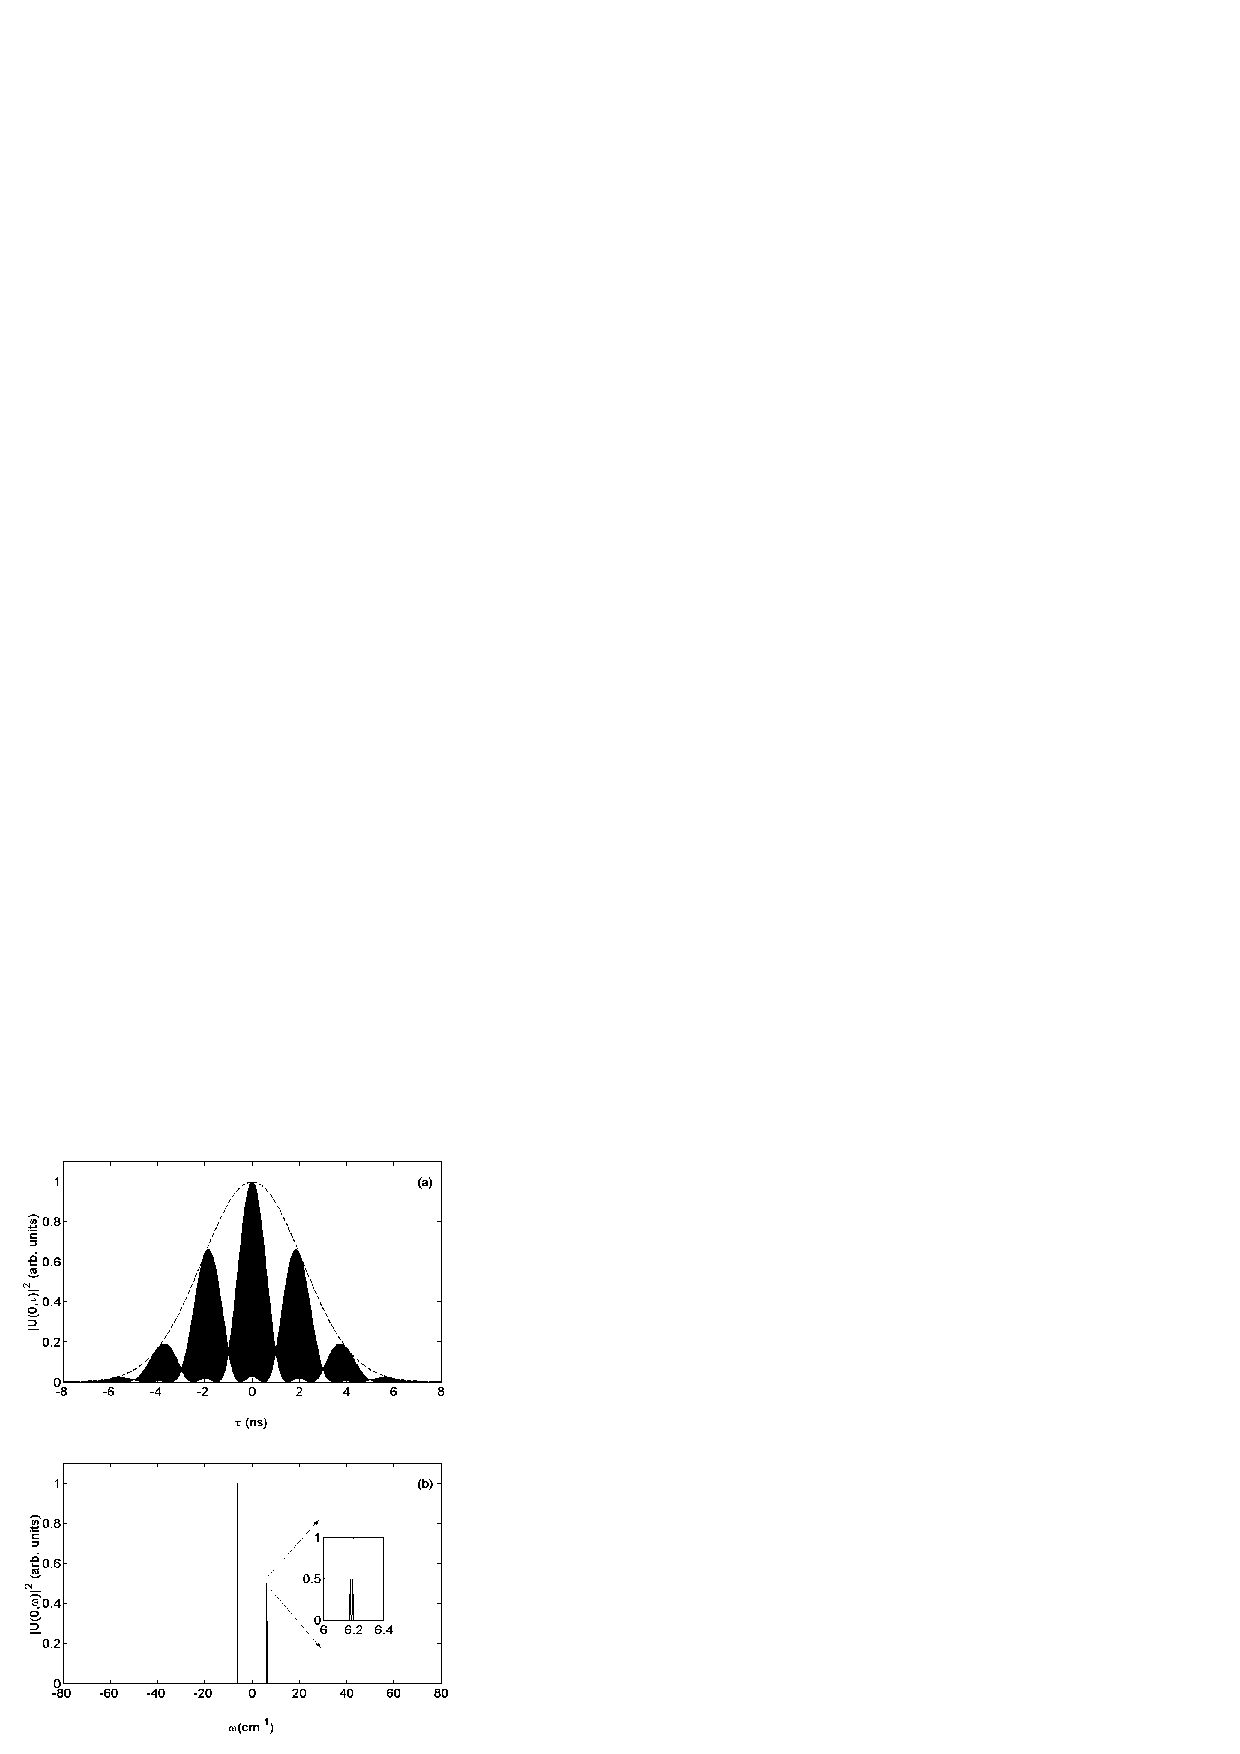
\includegraphics[width=5in]{nlsetime.pdf}
\end{center}
\renewcommand{\baselinestretch}{1}
\small\normalsize
\begin{quote}
\caption[Multimode pulse input toe NLSE]
{Multimode pulse input to the NLSE: (a) input pulse in time
domain and (b) input spectrum.}
\label{figA.1}
\end{quote}
\end{figure}
\renewcommand{\baselinestretch}{2}
\small\normalsize

The basic form of the initial complex wave envelope function is
%A.10
\begin {equation}
U(0,\tau) = exp \left( - {\tau^2 \over 2\tau_p^2} \right)
\left\{
\begin{array}{l}
exp\left( {i\Omega\tau \over 2} \right) + \\
exp\left( - {i\Omega\tau \over 2} \right)
\end{array}
\right\} ,
\end{equation}
where $\tau_p$ is the pulse width T$_p$ =5\,ns FWHM, normalized to the time scale
T$_0$, $\Omega$=366\,GHz is the frequency detuning between the two laser
sources normalized to a frequency scale $\Omega_0$ = 62.5\,MHz.  Figure A.1(a)
shows a plot of this pulse $|U(0,\tau)|^2$. The overall Gaussian envelope
has an FWHM of 5\,ns, the closely spaced dark lines are due to the 366\,GHz
($\sim$3\,ps) beating between the two input pump frequencies. The 2\,ns
modulations on the pulse are due to the 0.5\,GHz mode-structure in the
blue-shifted pump wave. Figure A.1(b) shows the input spectrum of this pulse
which consists of two highly monochromatic pump waves with a detuning of
$\Omega$=366\,GHz. The spectrum of the blue-shifted pump, upon magnification,
is seen to be composed of two very closely spaced peaks, with a separation of
$\Delta\nu$=0.5\,GHz. Hart {\it et al}.\ \cite{hart1} did not use pulsed
wave functions in their NLSE simulations as the size of the FFT required to do
so made it computationally prohibitive at that time. The size of the FFT was
chosen such that it would accommodate a time span of 16\,ns in order to go
sufficiently far into the wings on the Gaussian pulse; and a frequency span of
16\,THz in order to accommodate all the sidebands generated and prevent
spurious effects due to the reflection boundary conditions implicit in the
SSFM algorithm. These considerations dictated the size of the FFT to be
$\geq$(16 THz)$\cdot$(16 ns) = 256000. The nearest power of 2 is
2$^{18} = 262144$, which has been used throughout the present work. The
incorporation of the pulsed nature of the light was found to be necessary in
explaining the dynamics. From the perspective of the coupled amplitude
equations used by Hart {\it et al}.\ \cite{hart1}, the present model is equivalent
to a coupled-ODE model with $2^{18}$ coupled ODEs.

%Figure A.2
\begin{figure}
\begin{center}
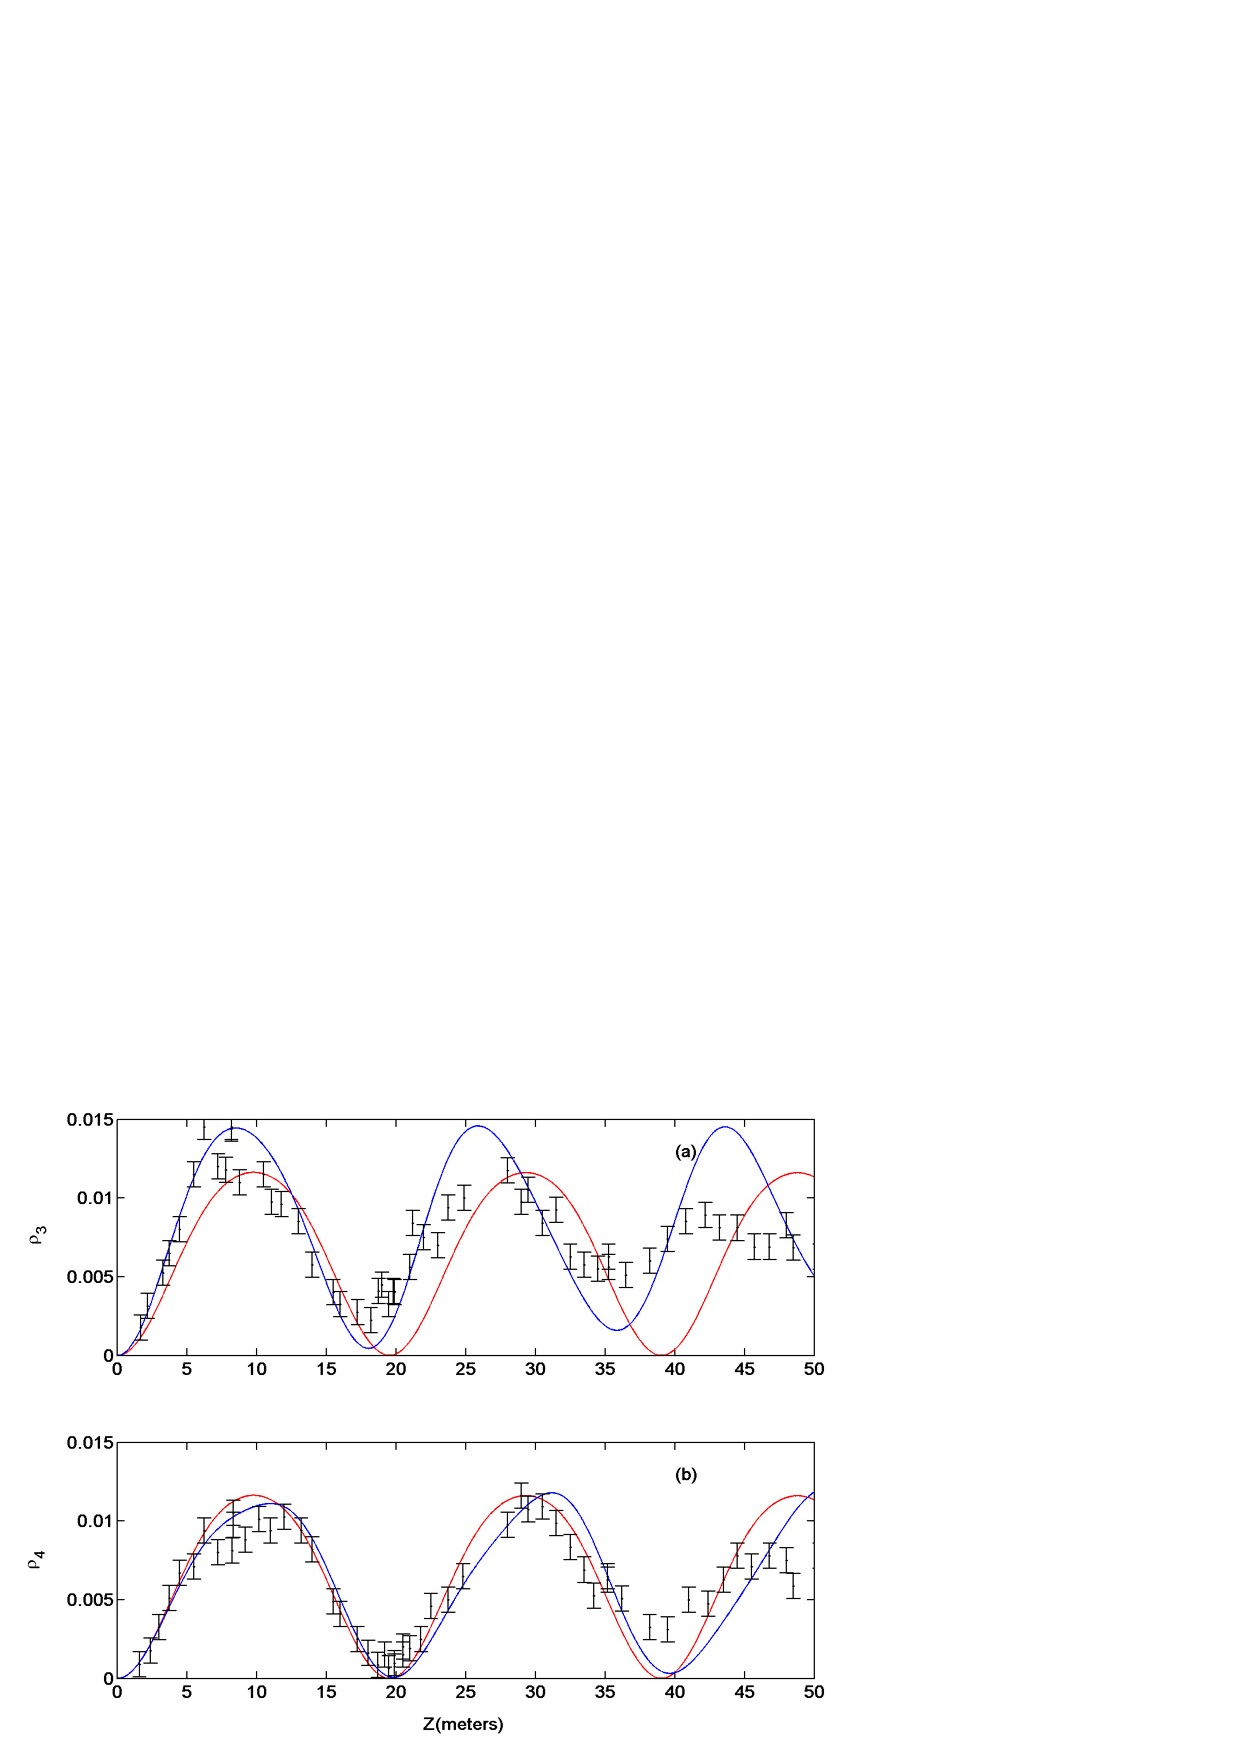
\includegraphics[width=5in]{modestruc21ornot.pdf}
\end{center}
\renewcommand{\baselinestretch}{1}
\small\normalsize
\begin{quote}
\caption[Short caption for Figure A.2.]
{Effects of inclusion of the multimode nature ($\Delta\nu = 0.5$\,GHz) of the blue-shifted input pump laser on the 1st order sideband evolution as a function of fiber length for P$_0 = 2.1$\,W. Dashed curves represent simulations without the multimode nature and solid curves represent simulations with the multimode nature. $\Omega = 366$\,GHz, $\gamma = 0.019$\,W$^{-1}$\,m$^{-1}$, and $\beta^{(2)} = 55$\,ps$^2$/km (a) power in the blue-shifted sideband, (b) power in the red-shifted sideband.}
\label{figA.2}
\end{quote}
\end{figure}
\renewcommand{\baselinestretch}{2}
\small\normalsize

%Figure A.3
\begin{figure}
\begin{center}
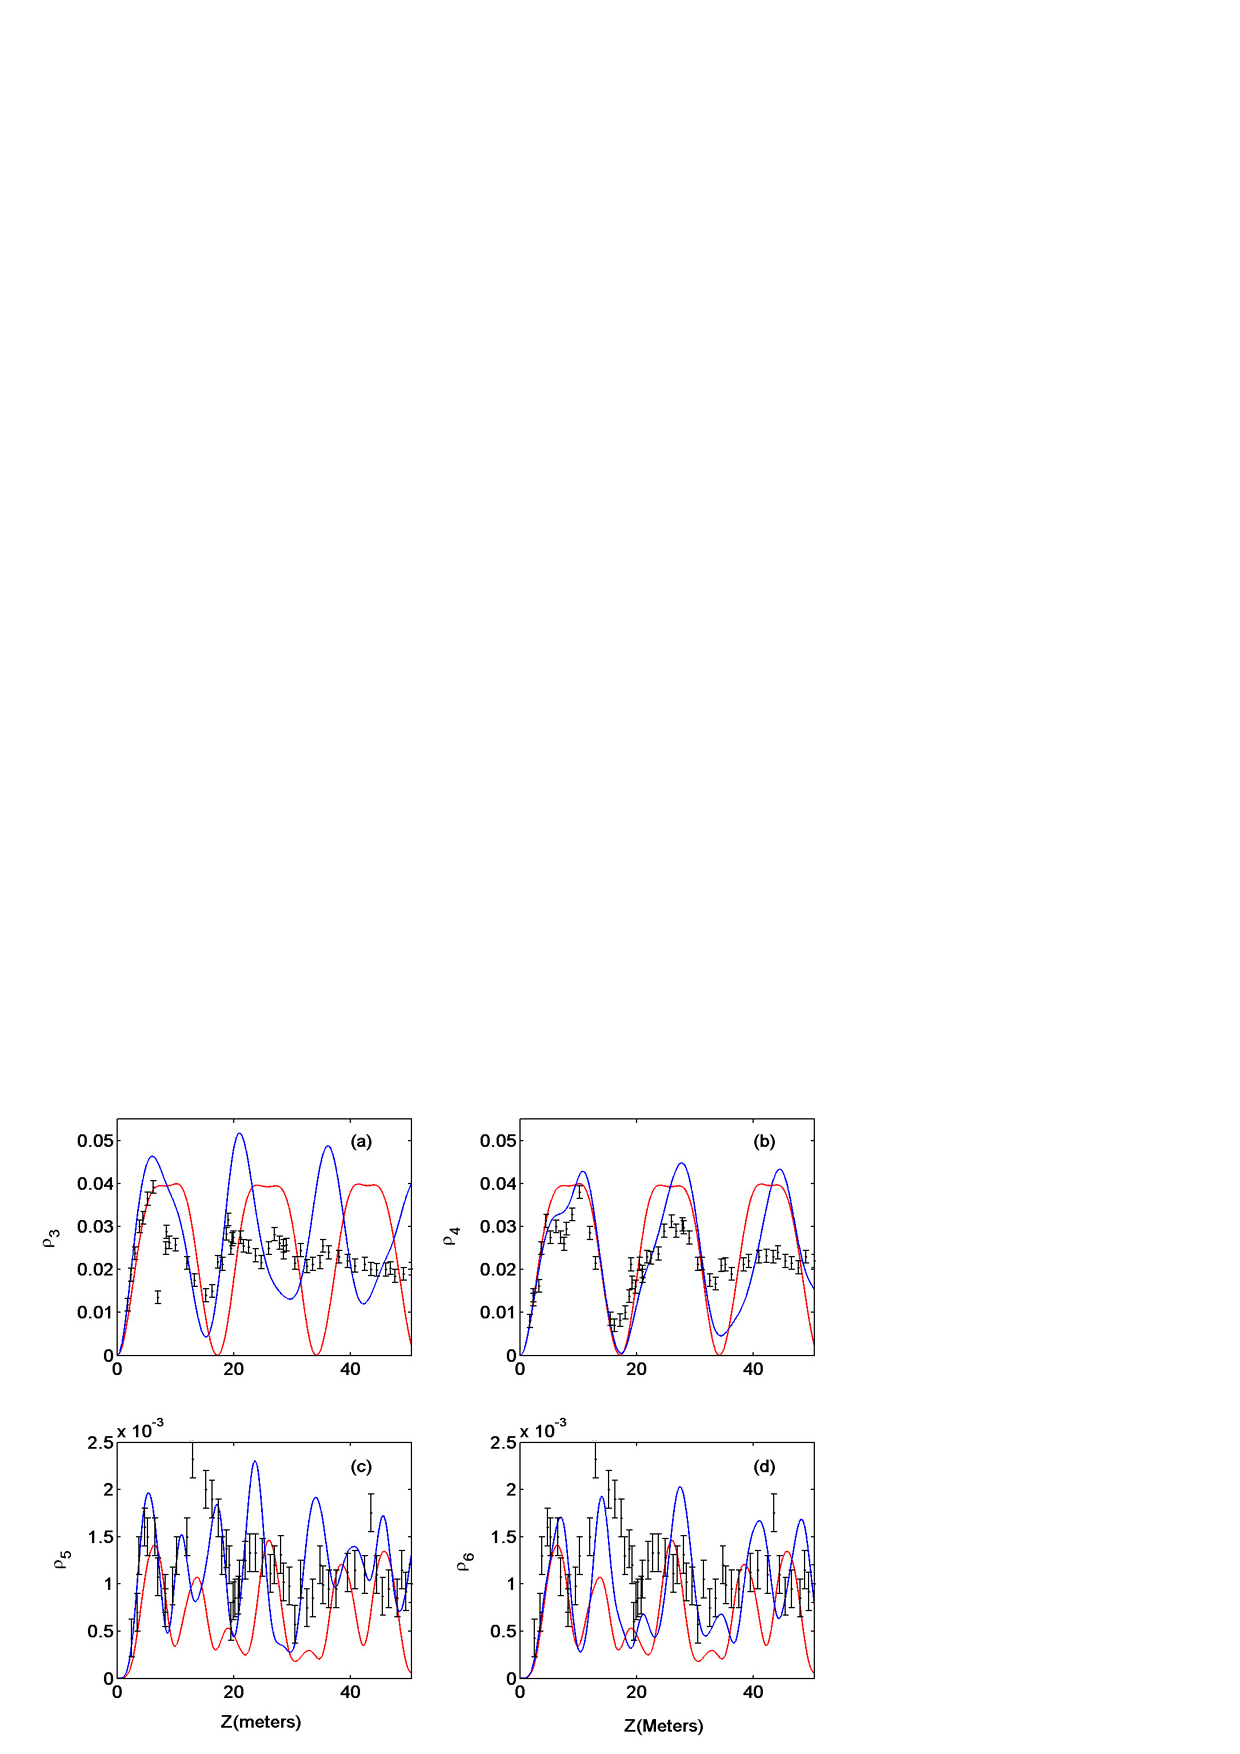
\includegraphics[width=5in]{modestruc55ornot.pdf}
\end{center}
\renewcommand{\baselinestretch}{1}
\small\normalsize
\begin{quote}
\caption[Effects of inclusion of the multimode nature]
{Effects of inclusion of the multimode nature ($\Delta\nu = 0.5$\,GHz) of the blue-shifted input pump laser on the 1st order sideband evolution as a function of fiber length for P$_0 = 5.5$\,W. Dashed curves represent simulations without the multimode nature and solid curves represent simulations with the multimode nature. $\Omega = 366$\,GHz, $\gamma = 0.019$\,W$^{-1}$\,m$^{-1}$, and $\beta^{(2)} = 55$\,ps$^2$/km (a) power in the first-order blue-shifted sideband, (b) power in the first-order red-shifted sideband, (c) power in the second-order blue-shifted sideband, (d) power in the second-order red-shifted sideband.}
\label{figA.3}
\end{quote}
\end{figure}
\renewcommand{\baselinestretch}{2}
\small\normalsize

%Figure A.4
\begin{figure}
\begin{center}
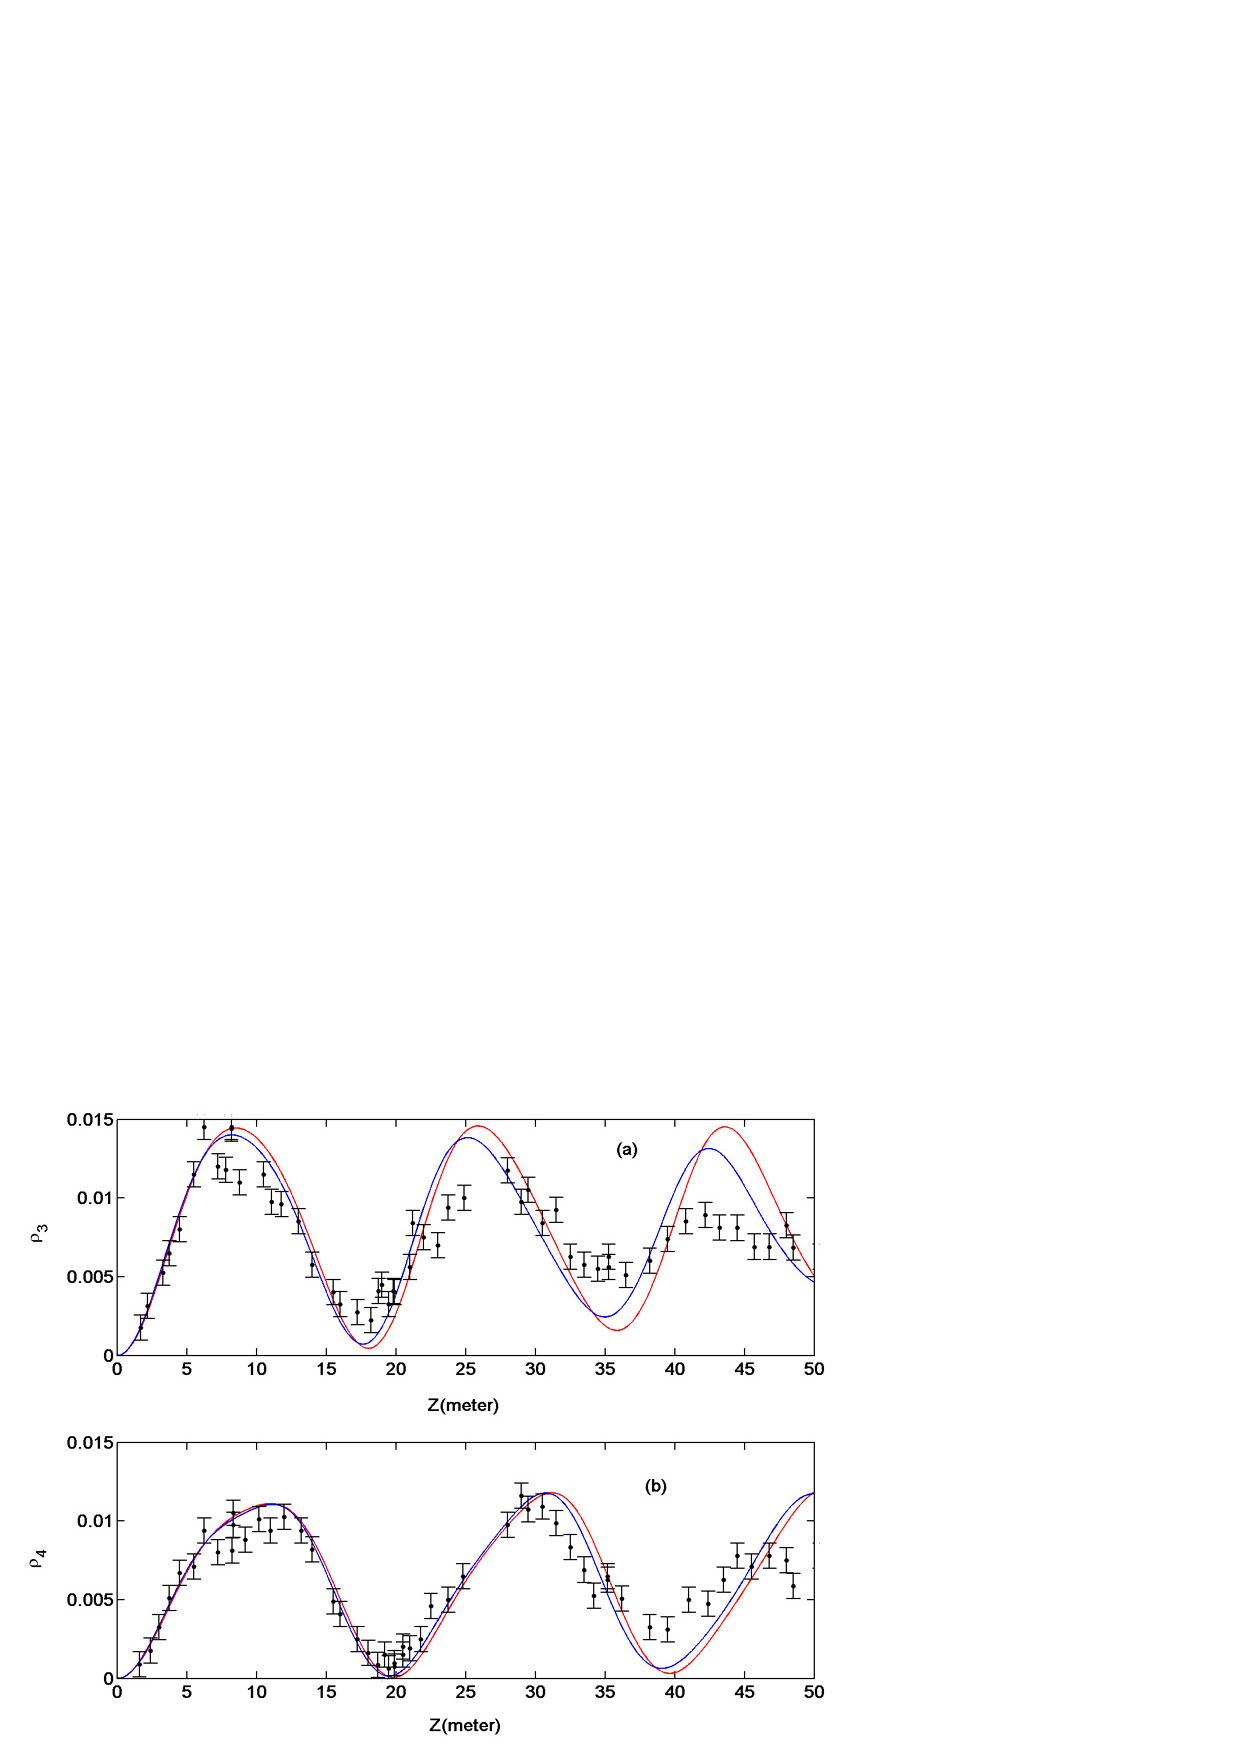
\includegraphics[width=5in]{nlsez21cwpulse.pdf}
\end{center}
\renewcommand{\baselinestretch}{1}
\small\normalsize
\begin{quote}
\caption[Effects of inclusion of the pulsed nature]
{Effects of inclusion of the pulsed nature (5\,ns FWHM) of the input pump laser light on the first-order sideband evolution as a function of fiber length for P$_0 = 2.1$\,W. Dashed curves represent cw simulations and solid curves represent pulsed simulations. $\Omega = 366$\,GHz, $\Delta\nu = 0.5$, $\gamma = 0.019$\,W$^{-1}$m$^{-1}$, and $\beta^{(2)} = 55$\,ps$^2$/,km (a) power in the blue-shifted sideband, (b) power in the red-shifted sideband.}
\label{figA.4}
\end{quote}
\end{figure}
\renewcommand{\baselinestretch}{1}
\small\normalsize

%Figure A.5
\begin{figure}
\begin{center}
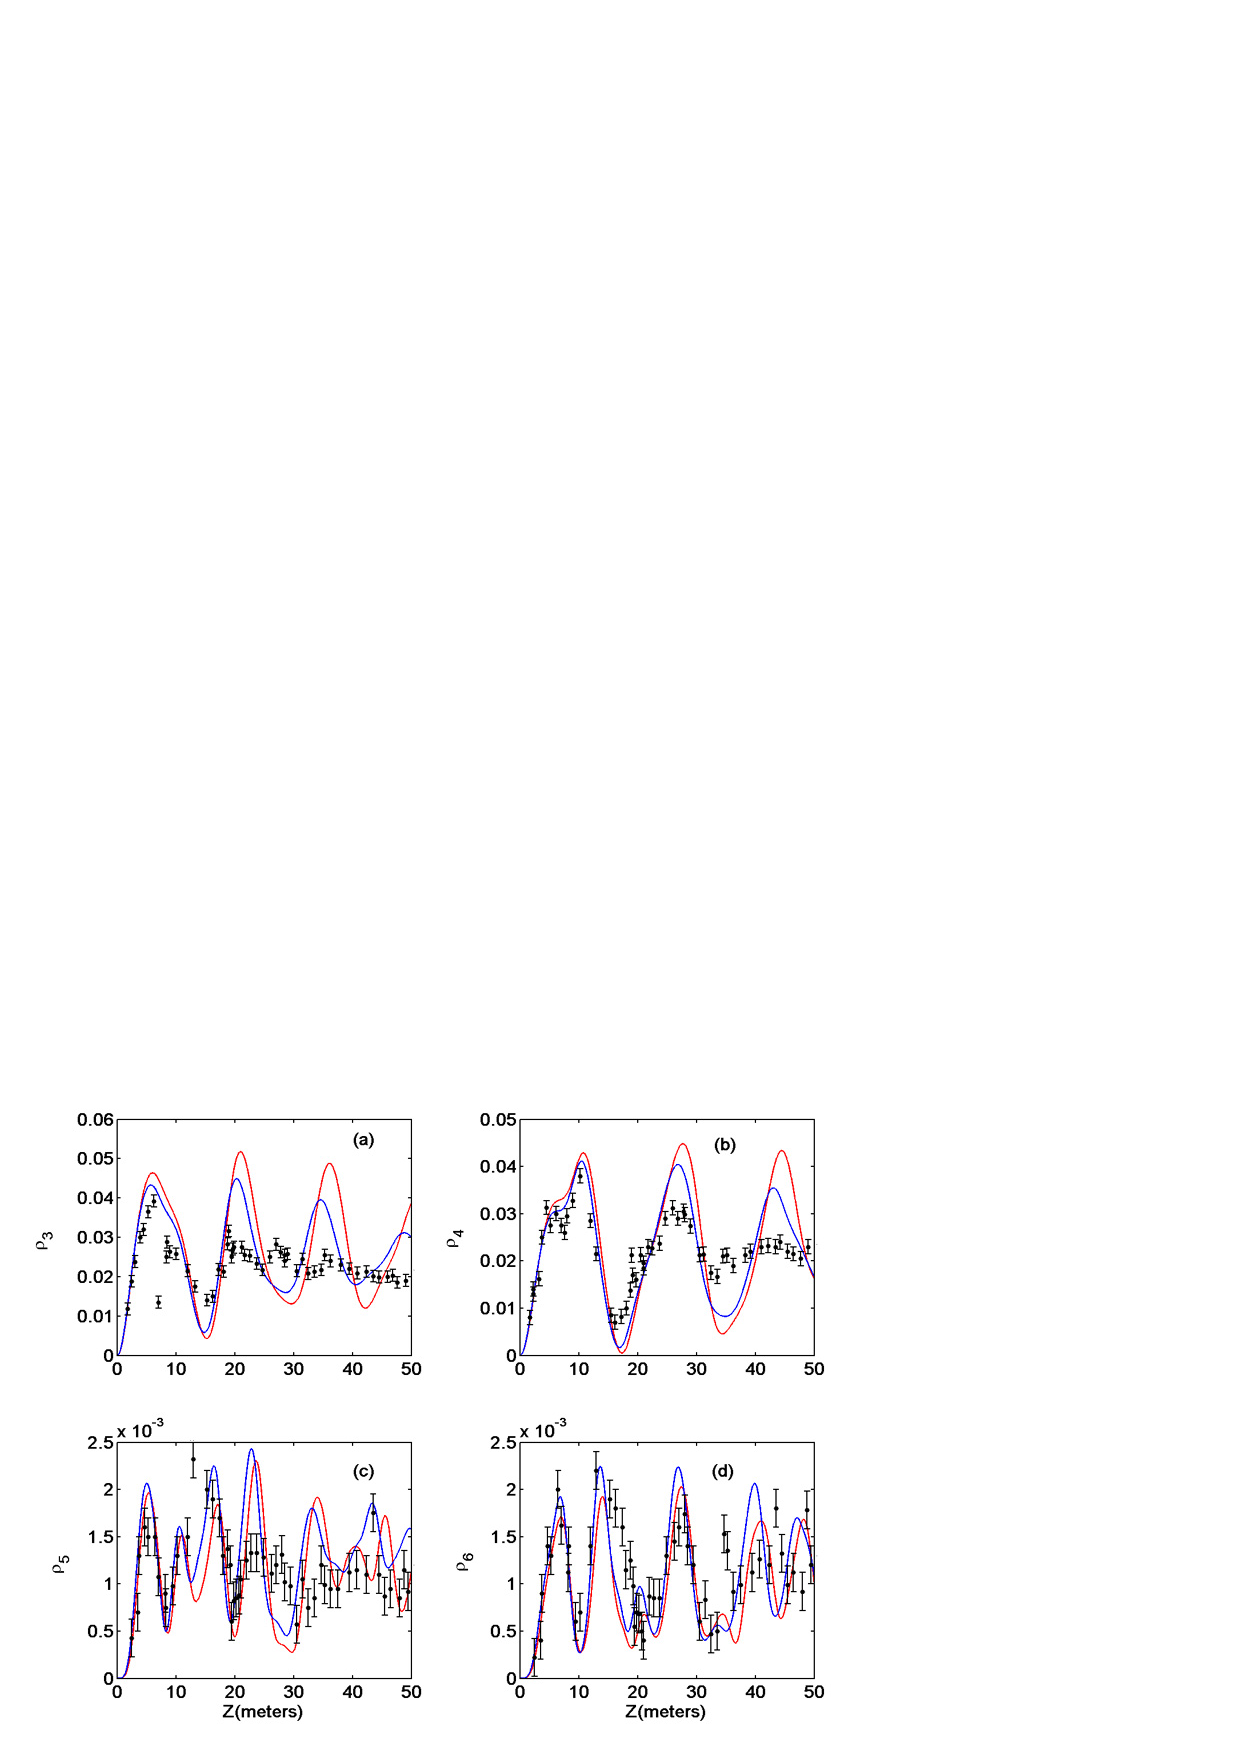
\includegraphics[width=5in]{nlsez55cwpulse.pdf}
\end{center}
\renewcommand{\baselinestretch}{1}
\small\normalsize
\begin{quote}
\caption
[Other effects of inclusion of the pulsed nature]
{Effects of inclusion of the pulsed nature (5\,ns FWHM) of the input pump laser on the first- and second-order sideband evolution as a function of fiber length for P$_0 = 5.5$\,W. Dashed curves represent cw simulations and solid curves represent pulsed simulations. $\Omega = 366$\,GHz, $\Delta\nu = 0.5$, $\gamma = 0.019$\,W$^{-1}$m$^{-1}$, and $\beta^{(2)} = 55$\,ps$^2$/,km (a) power in the first-order blue-shifted sideband, (b) power in the first-order red-shifted sideband, (c) power in the second-order blue-shifted sideband, (d) power in the second-order red-shifted sideband.}
\label{figA.5}
\end{quote}
\end{figure}
\renewcommand{\baselinestretch}{2}
\small\normalsize

Upon incorporation of the multimode nature of the blue input pump laser source
and the stochastic fluctuations in the initial power in the lasers, the
initial wave function takes the form
%A.11
\begin{equation}
U(0,\tau) = exp\left( - {\tau^2 \over 2\tau_p^2} \right)
\left\{
\begin{array}{l}
\sqrt{{1 + \delta\rho_1 \over 2}}
\left[ \begin{array}{l}
exp \left( {i(\Omega+\Delta\nu)\tau \over 2} \right) + \\
exp \left( {i(\Omega-\Delta\nu)\tau \over 2} \right)
\end{array} \right]\\
+ \sqrt{1 + \delta\rho_2} exp\left( - {i\Omega\tau \over 2} \right)
\end{array}
\right\}.
\end{equation}

\

\noindent $\Delta\nu = 0.5$\,GHz is the frequency separation between the two longitudinal
modes in the blue-shifted pump. $\delta\rho_1$ and $\delta\rho_2$ are
Gaussian random deviates (generated using the Box-Muller algorithm
\cite{boxmuller}) that represent the initial power fluctuations in each of the
pump laser sources. Their standard deviations were taken to be,
$\sigma_{\rho_1} = 0.2$, $\sigma_{\rho_2} = 0.11$ for simulations from 0\,m to
20\,m, $\sigma_{\rho_1} = 0.12$, $\sigma_{\rho_2} = 0.05$ for simulations from
20\,m to 50\,m along the length of the fiber. This is exactly the same
prescription used by Hart {\it et al}.\ \cite{hart1} in their simulations and is
dictated by their experimental measurements of the fluctuations in the pump
laser intensities.

At this point it is worth noting the effects of the inclusion of two attributes of
the input laser light, namely, the multimode nature of the blue-shifted pump, and
the pulsed nature of the input light (assumed to be cw in the simulations reported by
Hart {\it et al}.\ \cite{hart1}).

Figure A.2 shows a comparison between simulations with (solid curves) and without (dashed curves) the multimode nature for an input pump power of 2.1 Watts. The simulations with the mode structure show the asymmetry between the blue- and red-shifted sideband evolution, in particular, the difference in spatial wavelength between the two, and a non-return to zero nature of the evolution, as observed in the experimental data (black dots with error bars). These features are absent in the simulations without mode-structure. $\rho_3$ and $\rho_4$ stands for the first order blue- and red-shifted sidebands respectively.  Figure 2.3 shows the corresponding comparison for the case of 5.5 Watts of input pump power.  Here, too, the simulations incorporating the multimode nature of the blue-shifted pump (solid curves) are seen to be an improvement over those not incorporating it (dashed curves). A feature of the experimental data (black dots with errorbars) is that for the $\rho_3$ sideband, the initial part of the evolution involves a peak followed by a shoulder, while for the $\rho_4$ sideband, the initial part of the evolution involves a shoulder followed by a peak. This feature, too, is seen to occur as a result of the inclusion of the multimode nature of the blue-shifted pump.

The effect of inclusion of the pulsed nature of the input beam is seen in Fig.\ A.4 (for the 2.1 Watt case) and Fig.\ A.5 (for the 5.5 Watt case). The solid dashes represent simulations for a cw input beam and the solid curves represent those for a pulsed input beam. The incorporation of the pulsed nature clearly results in damping of the sideband trajectories which are seen to come closer to the experimental data \cite{hart1} (black dots with error bars).

Use of the FFT algorithm makes evaluation relatively fast compared to other
finite-difference schemes. The computational error is $O(\Delta z^2)$, thus
the solution converges with decreasing spatial step-size $\Delta z$.

The simulations were tested for the conservation of total power along the
fiber length (by setting the loss $\alpha$ to zero) and for the conservation
of asymmetry \cite{thompson1,hart1} given by
%A.12
\begin{equation}
C(Z) = \sum_{i=1}^{\infty}(2i-1)[\rho_{2i-1}(Z)-\rho_{2i}(Z)] .
\end{equation}

A clearer picture of the evolution of the sidebands is obtained by plotting both the
power in the sidebands and their standard deviations as a function of length along the fiber. Figures A.6(a) and A.6(b) show a comparison between simulation and experiment of the evolution
of the first-order blue-shifted ($\rho_3$) and red-shifted ($\rho_4$) sidebands,
respectively, for an input power of 2.1 W. The dashed curves represent NLSE simulations
which include the stochastic nature of the input powers of the pump lasers but exclude
the stochastic phase fluctuations added along the length of the fiber, an attribute
which is included in the simulations represented by the solid curves. The black dots
with error bars represent the experimental data. The measured sideband
power, normalized to the total power in the fiber, is periodic in length but
appears to be damping to a constant value. The measured data also show a clear
difference between the spatial wavelengths of oscillation of the blue-shifted ($\rho_3$) and red-shifted ($\rho_4$) sidebands trajectories, respectively. Both these features are captured well by both the simulations. Figures A.6(c) and A.6(d) compare experimental and simulated
measures of the evolution of the standard deviation in the sideband power
along the fiber length. It is clearly observed that simulations with phase noise
added to the light field along the length of the fiber (solid curves) are closer to the
experimental data as compared to those that exclude this feature (dashed curves). This indicates
the instrumental nature of the phase fluctuations in explaining key features of the dynamics.

%Figure A.6
\begin{figure}
\begin{center}
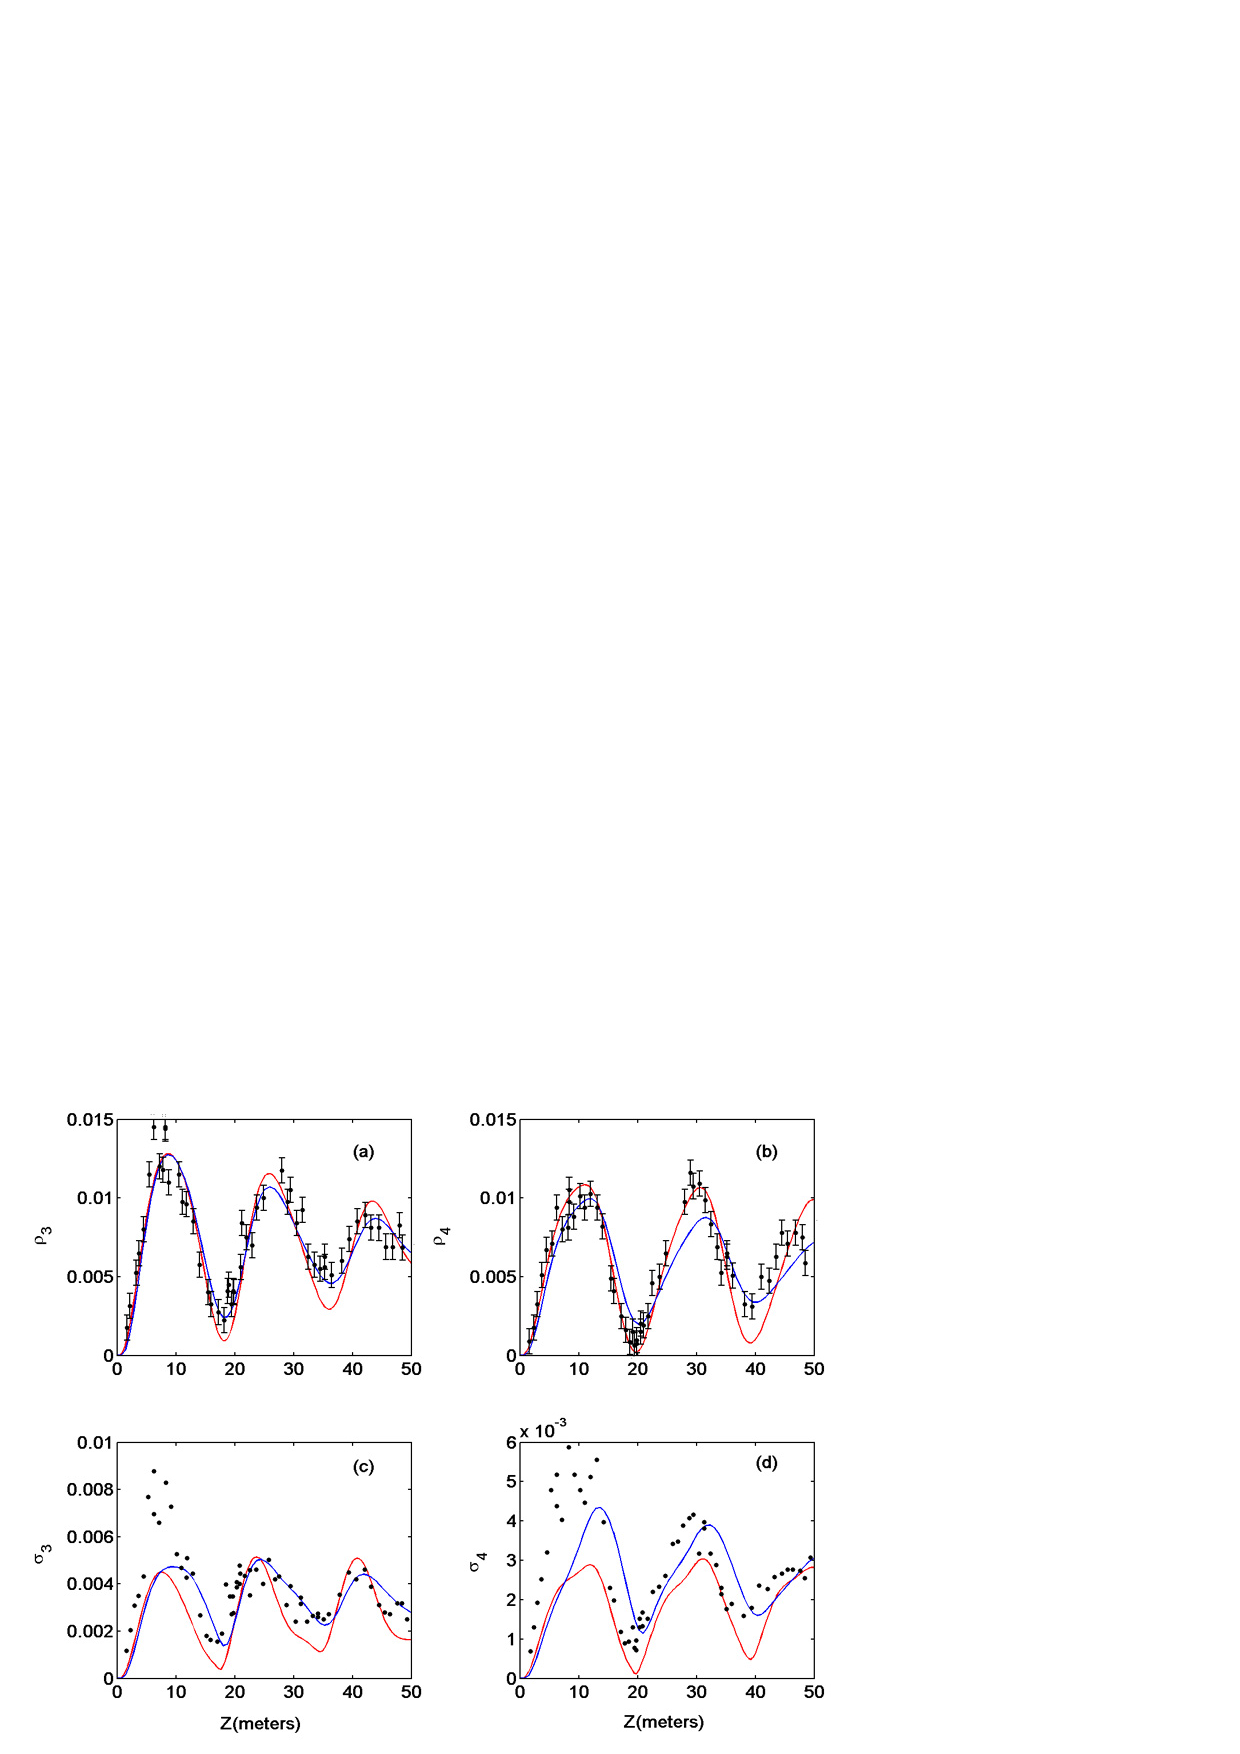
\includegraphics[width=5in]{nlsez21phaseornot.pdf}
\end{center}
\renewcommand{\baselinestretch}{1}
\small\normalsize
\begin{quote}
\caption
[Comparison between experiments measurements]
{Comparison between the experimental measurements \cite{hart1}(black), the random initial condition NLSE model excluding phase noise (dashed curves) and the stochastic phase noise NLSE model (solid curves) showing the first-order sideband evolution as a function of fiber length for P$_{0} = 2.1$\,W, $\Omega = 366$\,GHz, $\Delta\nu = 0.5$\,GHz,$\gamma = 0.019$\,W$^{-1}$m$^{-1}$, and $\beta^{(2)} = 55$ps$^2$/km: dynamical evolution of the: (a) power in the blue-shifted sideband, (b) power in the red-shifted sideband, (c) fluctuations in the blue-shifted sideband, (d) fluctuations in the red-shifted sideband.}
\label{figA.6}
\end{quote}
\end{figure}
\renewcommand{\baselinestretch}{2}
\small\normalsize

The apparent damping of the periodic sideband trajectory is seen more
dramatically in Figs.\ A.7(a) and A.7(b), which show the evolution of the
first-order sideband power along the fiber for an input power of 5.5\,W.
The two first-order sidebands evolve differently. They appear to
damp to a constant value at a faster rate than for the case with an input pump
power of 2.1\,W. Here again, NLSE simulations that incorporate phase noise along the length
of the fiber (solid curves) are much more successful in accurately capturing the dynamical features of the system than NLSE simulations that do not take this feature into account (dashed curves).  Figures A.7(c) and A.7(d) show a comparison between the simulated and measured standard deviations. Comparisons for the second-order blue-shifted ($\rho_5$) and red-shifted ($\rho_6$) sidebands, respectively, are shown in Figs.\ A.7(e) and A.7(f).


%Figure A.7
\begin{figure}
\begin{center}
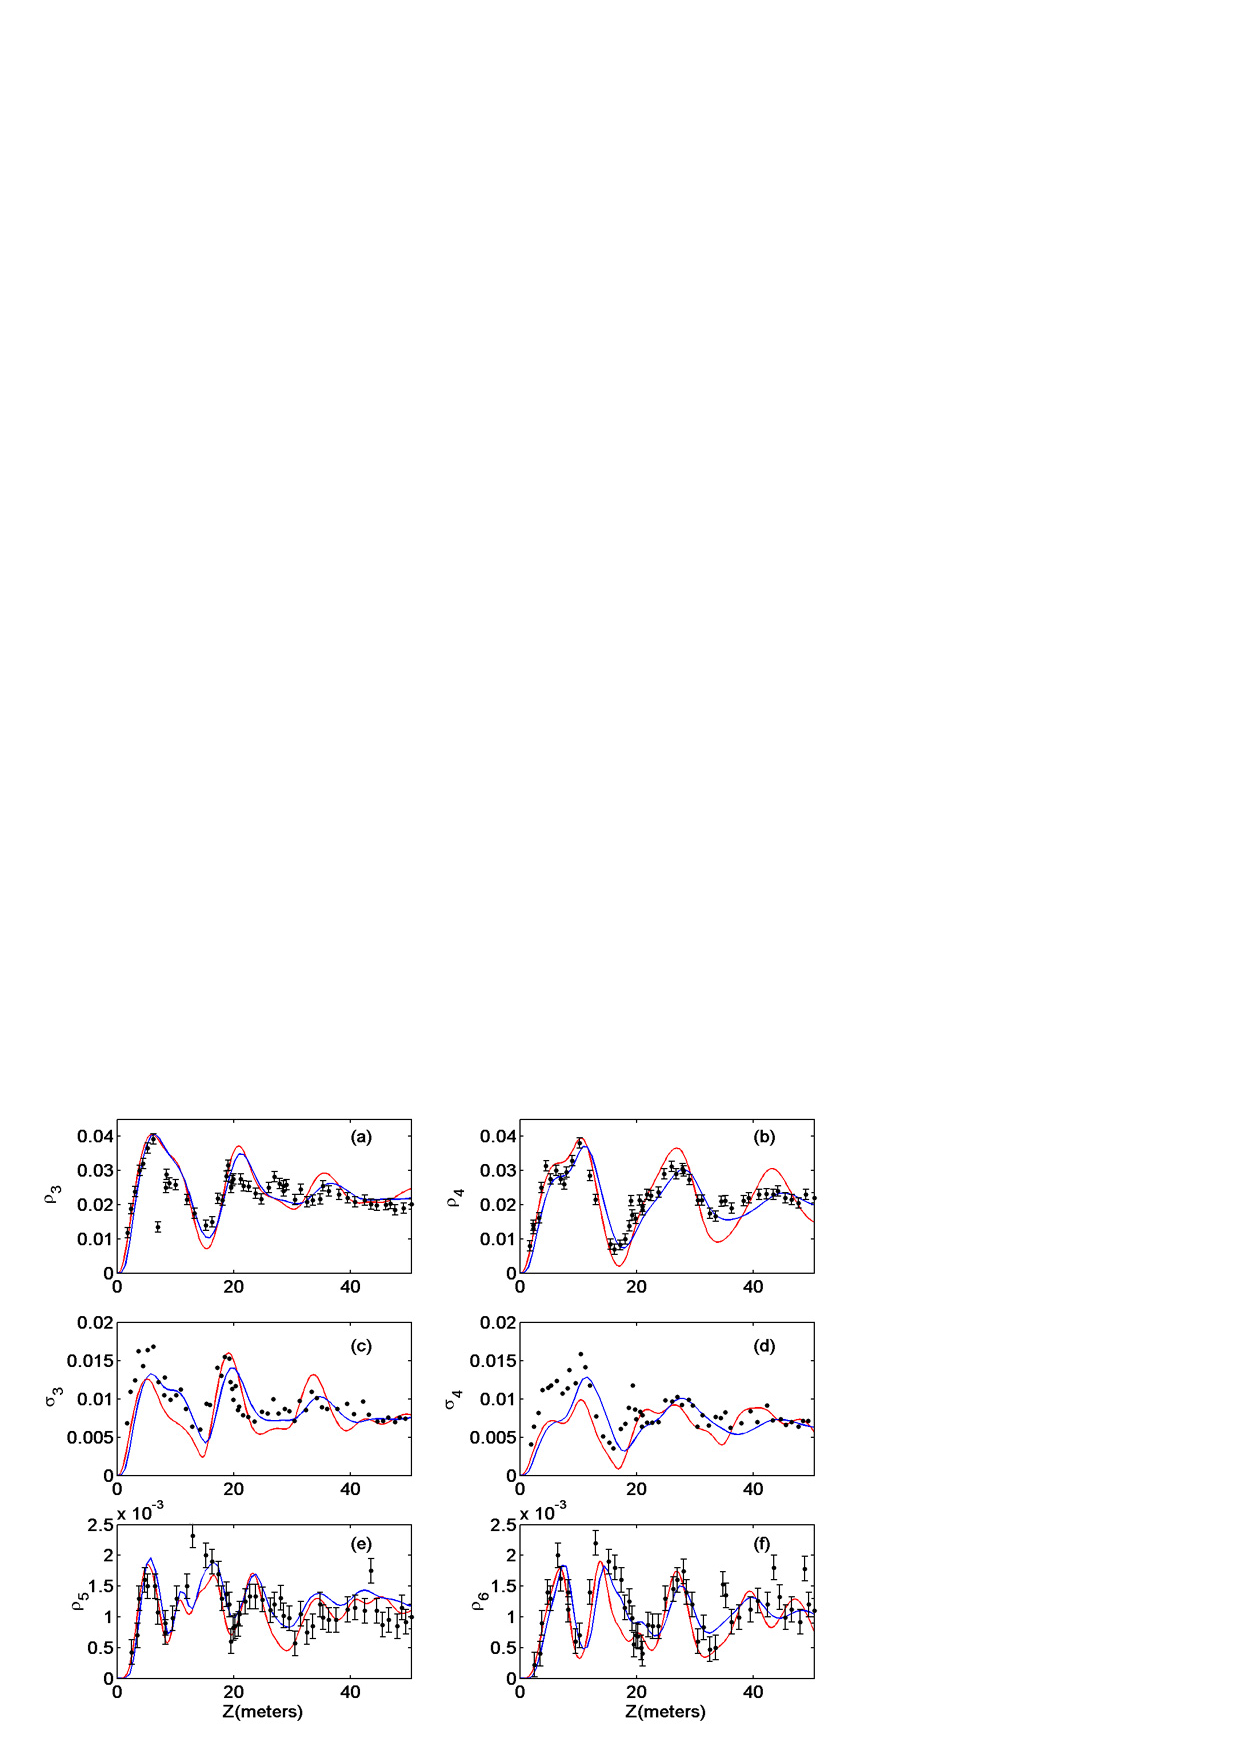
\includegraphics[width=5in]{nlsez55phaseornot.pdf}
\end{center}
\renewcommand{\baselinestretch}{1}
\small\normalsize
\begin{quote}
\caption
[This figure caption is indented and single-spaced]
{This figure caption is indented and single-spaced.  Comparison between the experimental measurements \cite{hart1} (black), the random initial condition NLSE model excluding phase noise (dashed curves) and the stochastic phase noise NLSE model (solid curves) showing the first- and second-order sideband evolution as a function of fiber length for P$_{0} = 5.5$\,W, $\Omega = 366$\,GHz, $\Delta\nu = 0.5$\,GHz, $\gamma = 0.019$\,W$^{-1}$m$^{-1}$, and $\beta^{(2)} = 55$\,ps$^2$/km: dynamical evolution of the: (a) power in the first-order blue-shifted sideband, (b) power in the first-order red-shifted sideband, (c) fluctuations in the first-order blue-shifted sideband, (d) fluctuations in the first-order red-shifted sideband, (e) power in the second-order blue-shifted sideband, (f) power in the second-order red-shifted sideband.}
\label{figA.7}
\end{quote}
\end{figure}
\renewcommand{\baselinestretch}{2}
\small\normalsize

The observed dynamical evolution of the sidebands is found to depend
sensitively on the strength of the stochastic phase fluctuations. Yet, best
agreement with the experimental results of Hart {\it et al}.\ \cite{hart1} is
achieved with exactly the same noise strength $\sigma^2_\phi$ as used in
their truncated ODE model, namely, $\sigma^2_\phi = 0.0067$\,m$^{-1}$. They
report that including phase noise in their FWM calculations resulted in a
spurious linear drift in the trajectories for the sideband power with length.
To remove this artifact of the computations, they added a linear loss to their
coupled ODEs. They set the loss coefficient $\alpha = 0.0046$\,m$^{-1}$ by
finding the value that removed this increasing slope. We have observed exactly
the same secular growth phenomenon for a wide range of the noise strength
$\sigma^2_\phi$ and have arrived at an empirical prescription for $\alpha$
namely, $\alpha\sim\sigma^2_\phi$, where $\sigma^2_\phi$ is the
variance of the added phase noise. This indicates the general nature of
dynamics resulting from the addition of stochastic, $\delta$-correlated phase
fluctuations to systems governed by nonlinear partial differential equations
\cite{risken}.

It is remarkable that the strength of the phase noise required is the same in
both the 2.1\,W and the 5.5\,W cases. Further, it is worth noting that exactly
the same noise strength was used by Hart {\it et al}.\ \cite{hart1}, the difference
being that they introduced phase noise only in the pump frequencies, whereas
we have introduced it in all the Fourier modes ($\sim2^{18}$). As a
confirmation of this result, they also performed experiments and numerical
simulations examining the sideband power dependence on the input power at a
fixed length of 50.4\,m of the same fiber. We have repeated these simulations
with the stochastic NLSE model and the results are shown in Figs.\ 2.8(a)
(blue-shifted sideband) and 2.8(b) (red-shifted sideband). The experimental
measurements of the sideband powers are represented by filled squares and the
results of numerical simulations are represented by triangles (without phase
noise) and by circles (with phase noise). The simulations are seen to follow
the general trend seen in the experiments. As the pump power is increased, the
triangles (without phase noise) start to disagree with experiment, whereas the
circles (with phase noise) are much closer to experiment. The phase noise
strength used in these simulations was exactly the same as that used in the
simulations depicted in Figs.\ A.6 and A.7. The agreement between the phase noise
simulations and the experimental data was (once again) highly sensitive to the
noise strength. Since this experiment (unlike those shown in Figs.\ A.2 - A.7)
is non-destructive, it can be used to deduce the strength of phase noise
processes in a given optical fiber. It will be shown in Sec.\ 2.4 that a
likely cause of the phase noise is fluctuation in the linear refractive index
of the fiber. The noise strength deduced from the present computational study
corresponds to a refractive index inhomogeneity of
$\langle \Delta n^{2} \rangle \sim 10^{-16}$.

%Figure A.8
\begin{figure}
\hspace{1.25in}
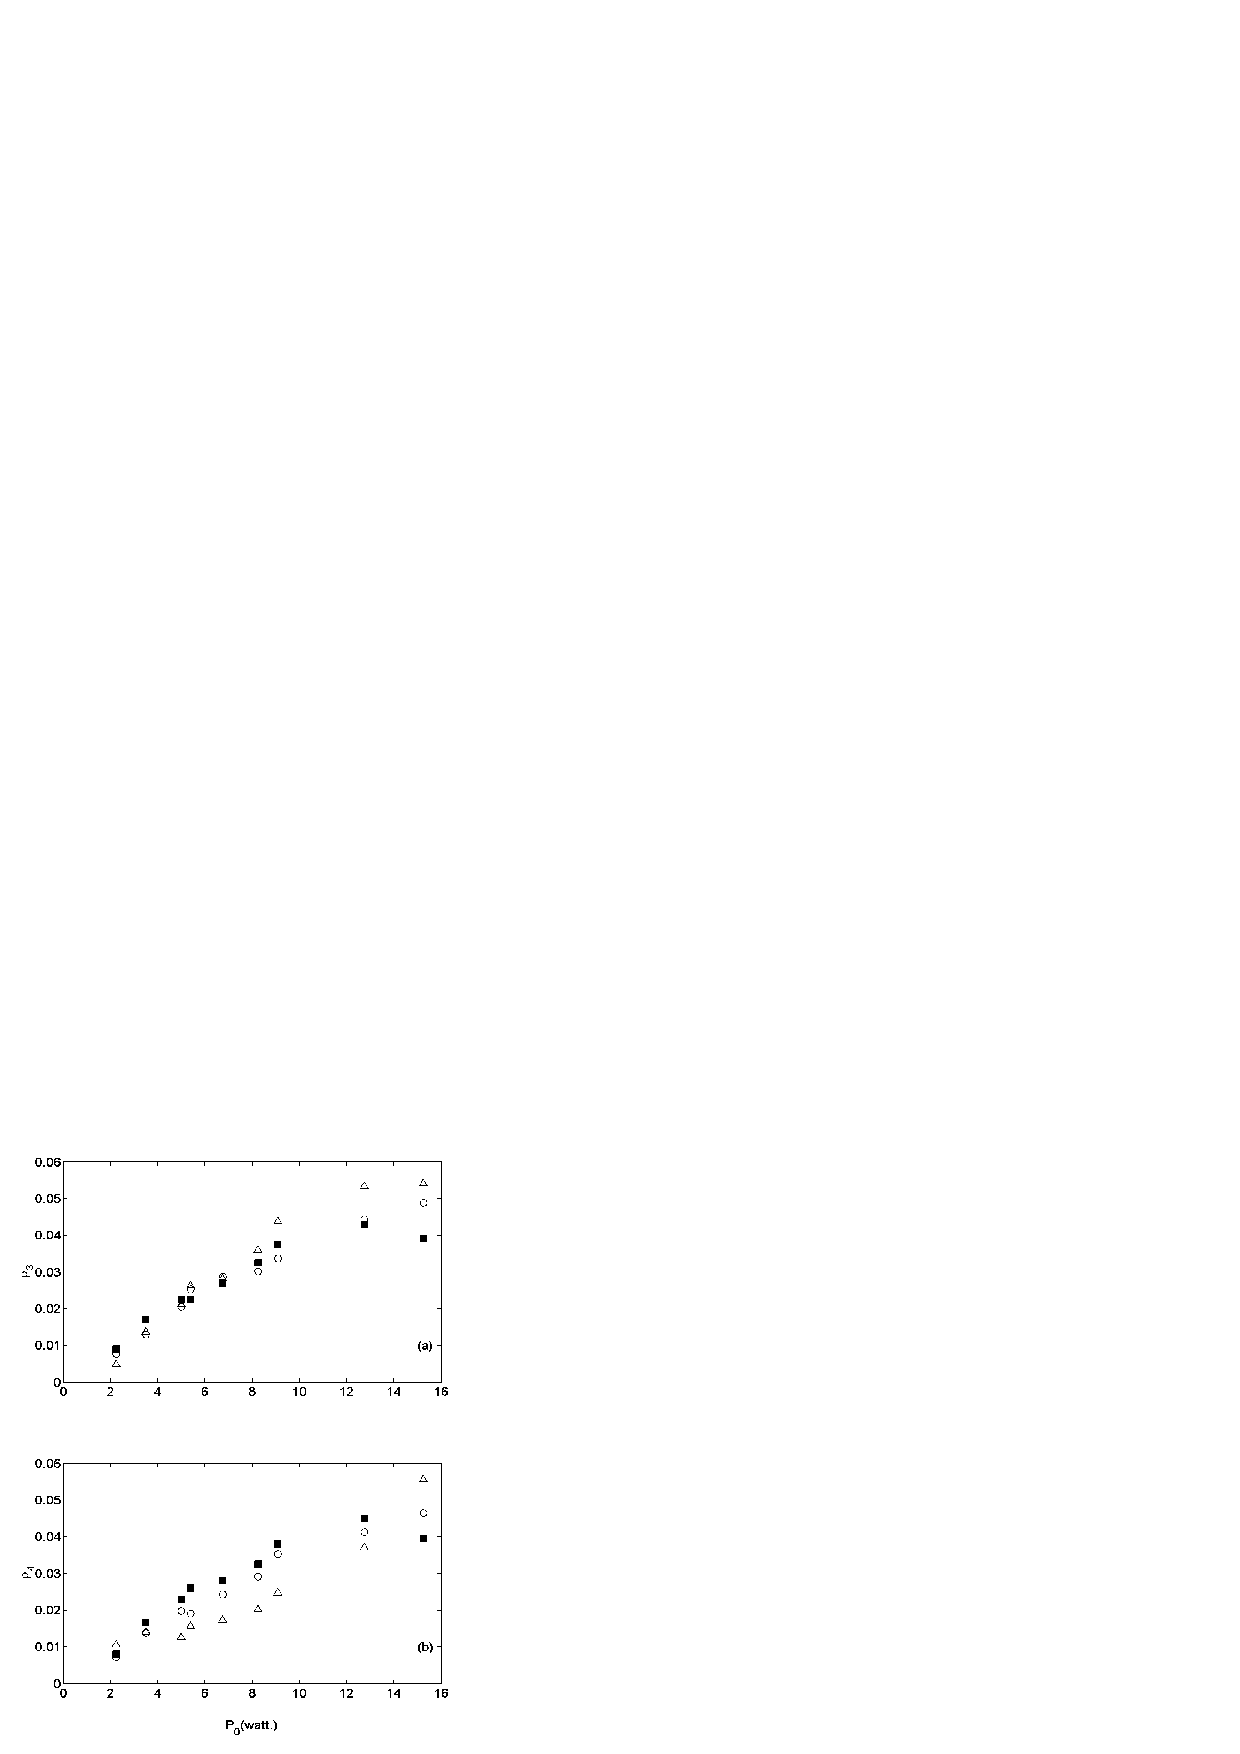
\includegraphics[width=5in]{nlsefinal.pdf}
\renewcommand{\baselinestretch}{1}
\small\normalsize
\begin{quote}
\caption
[Comparison between the experiments measurements (filled squares)]
{Comparison between the experimental measurements (filled squares), simulations without stochastic phase fluctuations (open triangles) and with stochastic phase fluctuations (open circles) of the first-order sideband power versus pump input power for L=50.39\,m, and $\Omega = 366$\,GHz: power in the (a) blue-shifted sideband and (b) red-shifted sideband.}
\label{figA.8}
\end{quote}
\end{figure}
\renewcommand{\baselinestretch}{2}
\small\normalsize

%Figure A.9
\begin{figure}
\begin{center}
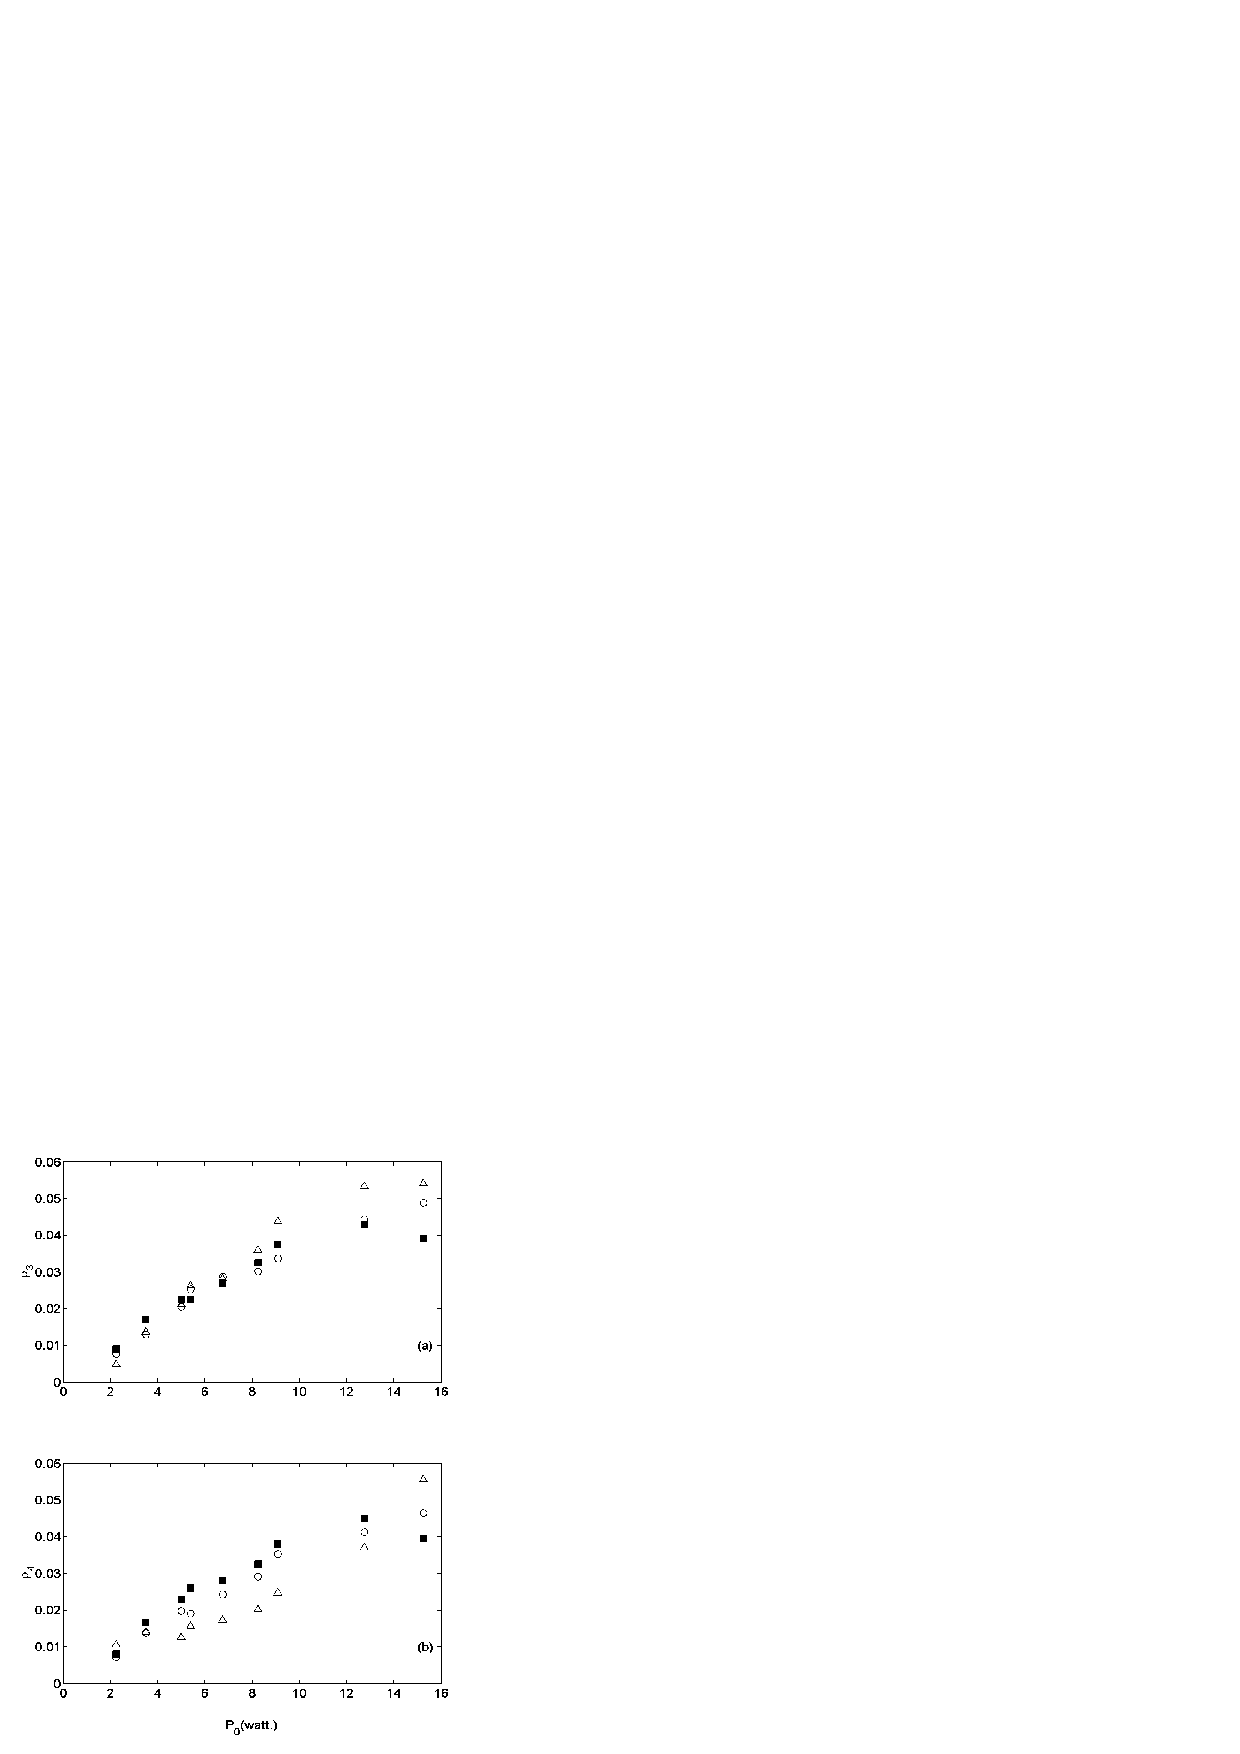
\includegraphics[width=5in]{nlsefinal.pdf}
\end{center}
\renewcommand{\baselinestretch}{1}
\small\normalsize
\begin{quote}
\caption
[Evolution of the FWM spectrum]
{Evolution of the FWM spectrum along the fiber (a) P=2.1\,W, experiment, (b) P=5.5\,W, experiment, (c) P=2.1\,W, stochastic-NLSE model, (d) P=5.5\,W, stochastic-NLSE model.}
\label{figA.9}
\end{quote}
\end{figure}
\renewcommand{\baselinestretch}{2}
\small\normalsize

Till now the comparisons between our simulations of the full NLSE and the
truncated ODE model give basically the same results, although with much better
agreement with experiment. However, the full NLSE can also provide a detailed
comparison with the experimental spectra. This was not available from the
truncated ODE model. The simulations reported in this work were carried out
with a very high frequency and time resolution in order to incorporate the
fact that the input light was not cw, but was composed of $\sim$ 5\,ns long
pulses; and that the number of sidebands generated required the frequency
spread of the FFT to be $\sim$ 16\,THz, while resolving a longitudinal
mode-structure of $\Delta\nu$ $\sim 0.5$\,GHz. The spectral resolution used was
$\sim$ 0.05\,GHz, whereas the spectrometer used to observe the spectra had a
resolution 1000 times larger ($\sim$ 50\,GHz). To account for this difference,
the simulated spectra were first convolved with a Gaussian of unit peak and
62\,GHz FWHM, before they were compared with the observed spectra.

Figures A.9(a) and A.9(b) show three-dimensional plots of the average experimental
FWM output spectrum along the length of the fiber for input pump powers of 2.1\,W and 5.5\,W,
 respectively (courtesy Hart {\it et al}.\ \cite{hart1}). The vertical
axis represents the intensity, normalized to the peak power in one of the
input pumps, plotted on a logarithmic scale. The pump frequencies are centered
on $+/-\Omega/2$ and the fiber length is increasing into the page. Figures
9(c) and 9(d) show the corresponding comparisons based on simulations using
the stochastic-NLSE model. The basic features of the spectral evolution are
captured by the simulations.

%Figure  A.10
\begin{figure}
\begin{center}
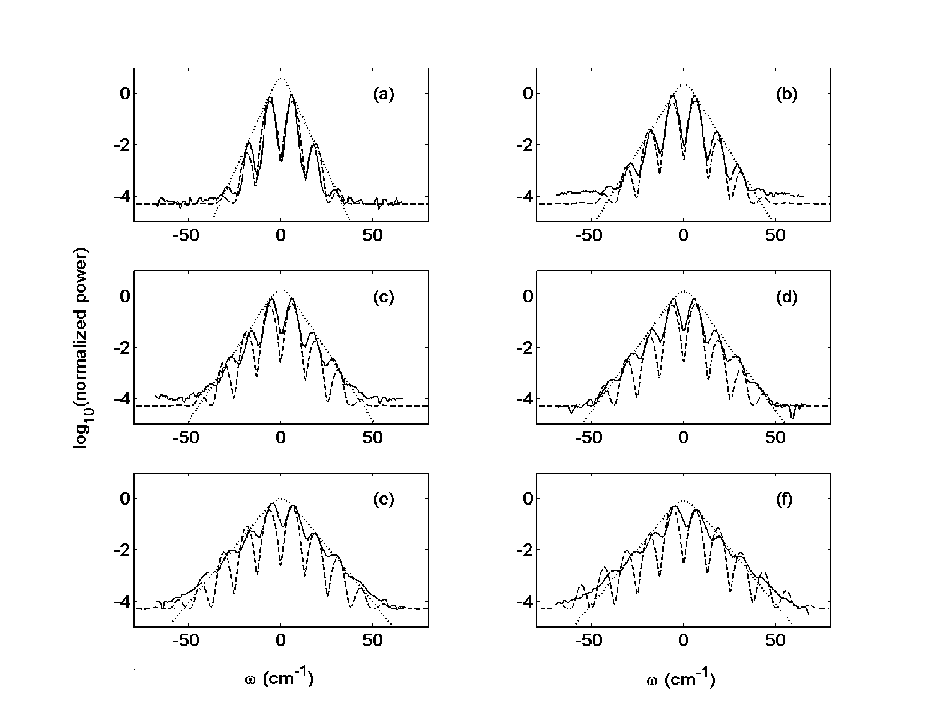
\includegraphics[width=5in]{nlsespec.eps}
\end{center}
\renewcommand{\baselinestretch}{1}
\small\normalsize
\begin{quote}
\caption
[Experimental FWM output spectrum]
{Experimental FWM output spectrum (solid line), convolved spectra from simulations of the stochastic NLSE model (dashed line), and hyperbolic secant envelope fit (dotted line) for pump input powers P$_0$ of (a) 2.1\,W, (b) 5.5\,W, (c) 6.7\,W, (d) 8.3\,W, (e) 12.7\,W, (f) 17.4\,W, fiber length L$= 50.39$\,m, $\Omega = 366$\,GHz, $\Delta\nu = 0.5$\,GHz, $\gamma = 0.019$\,W$^{-1}$m$^{-1}$, and $\beta^{(2)} = 55$\,ps$^2$/km.}
\label{figA.10}
\end{quote}
\end{figure}
\renewcommand{\baselinestretch}{2}
\small\normalsize

Hart {\it et al}.\ \cite{hart1} also documented the experimentally observed FWM
output spectra for a fixed fiber length of 50.39 meters for 6 different input
pump powers. They state the coefficients A and B of the hyperbolic secant
envelopes that best fit the output spectra which are given by
%A.13
\begin{equation}
f(\omega) = Asech(B\omega) ,
\end{equation}
where A and B are the experimental fit parameters.

The hyperbolic secant parameters A and B, that best fit the simulated spectra
are exactly the same as those that best fit the experimental spectra
\cite{hart1} for all the 6 cases of input power considered. Figure 2.10 shows an
overlap of the simulated spectra (dashed line), with the experimental spectra
(solid line) and the experimental hyperbolic secant envelope (dotted line) for
6 different pump powers, namely, (a) 2.1\,W, (b) 5.5\,W, (c) 6.7\,W, (d) 8.3\,W, (e)
12.7\,W, (f) 17.4\,W. The hyperbolic secant parameters for each of these pump
powers are (a) A=3.85 and B=0.36, (b) A=2.26 and B=0.27, (c) A=1.81, B=0.25,
(d) A=1.56 and B=0.23, (e) A=0.98,B=0.20, and (f) A=0.81 and B=0.20. The exact
shapes of the simulated spectra match very well with the experimental spectra
for low input pump powers (2.1\,W and 5.5\,W), but tend to lack the "filled-in"
character of the experimental spectra at higher powers (6.7\,W, 8.3\,W, 12.7\,W and
17.4\,W).

\section{Discussion}

Hart {\it et al}.\ \cite{hart1} postulated that strong candidates for the possible
physical sources of the phase fluctuations are stimulated Brillouin
scattering, stimulated Raman scattering and fiber medium inhomogeneities.
Brillouin scattering was eliminated as a source, since a backward propagating
wave, which is a signature of Brillouin scattering in optical fibers, was not
observed in the experiments. We have  modeled stimulated Raman scattering
\cite{Agrawal8, headley} for our system and have found no evidence to
support the hypothesis that it could be a possible source of the stochastic phase
fluctuations for fiber lengths up to 50 meters and pump power levels up to 5.5 Watts.
A more detailed discussion of the Raman scattering simulations performed is given in Chap.\ 3.
Apart from these, quantum phase fluctuations are another well
known, though extremely weak, source of phase noise in optical fibers
\cite{Agrawal2,perlmutter1}.

Fiber medium inhomogeneities were identified as the major cause of the
stochastic phase fluctuations. These inhomogeneities can manifest themselves
through spatial and/or temporal fluctuations in the fiber parameters, namely,
the linear refractive index $n_0$, the group velocity $v_g$, the group
velocity dispersion $\beta^{(2)}$ and the nonlinearity
$\gamma$ \cite{abdullaev}. Of these, the fluctuation in the linear refractive
index was found to be the only source of phase fluctuation that had a
significant effect on the dynamics. A relationship between the level of
refractive index fluctuations and the  corresponding level of phase
fluctuations has been arrived at. It is found that refractive index
fluctuations as small as $\sigma_n^2 \sim 10^{-17}$\,m$^{-1}$ can cause the
desired phase fluctuations. Possible sources of these refractive index
fluctuations are discussed below.

Consider the modified nonlinear Schr\"odinger equation (NLSE) which is
stated below, with the linear multiplicative noise term represented in terms of
spatial and temporal fluctuations in the refractive index of the fiber.
%A.14
\begin{equation}
{\partial U \over \partial z} + {i\beta^{(2)} \over 2T_0^2} {\partial^2U \over \partial\tau^2} + {\alpha U \over 2} + ik_0 \delta n(z,\tau)U - i\gamma P_{0}|U|^2 U = 0 ,
\end{equation}
where $\delta n(z,\tau)$ is the spatial and temporal variation of the refractive
index along the fiber. It can be caused by temperature and density
fluctuations in the fiber \cite{glenn}.

The thermodynamic estimate for $\Delta n$ is given by \cite{glenn}
%A.15
\begin{equation}
\langle \Delta n^{2} \rangle = {-kT\rho^2 \over V^2}
\left( {\partial V \over \partial P} \right)_{T}
\left( {\partial n \over \partial \rho} \right)_{T}^{2}
 + {kT^2 \over \rho VC_v} \left( {\partial n \over \partial T} \right)_{\rho}^2 .
\end{equation}

This gives the mean-square index fluctuation in terms of the properties of
the material. It can be rewritten as
%A.16
\begin{equation}
\langle \Delta n^{2} \rangle = {V_{\rho}+V_T \over V} = \langle \Delta n^{2} \rangle_{\rho}+\langle \Delta n^{2} \rangle_{T} .
\end{equation}

For a fiber of length z=1\,m and radius r=2.82\,$\mu$m
(Volume V=2.5 $\times 10^{-12}$\,m$^3$), these have been calculated to be
%A.17
\begin{eqnarray}
\langle \Delta n^2 \rangle_{\rho} \sim 10^{-21} & \equiv & \langle \Delta \rho^2 \rangle \sim 10^{-14}
{kg^2 \over m^6}, \nonumber \\
\langle \Delta n^2 \rangle_T \sim 10^{-23} & \equiv & \langle \Delta T^2 \rangle \sim 10^{-12}~{^\circ}C^2 .
\end{eqnarray}

It should be noted that $\langle \Delta n^2 \rangle \propto (1/z) \Rightarrow \delta n \propto  (1 / \sqrt{z})$. The corresponding phase fluctuation that this would lead to in the NLSE is given by $\delta \phi=k_{0} \delta n z \propto \sqrt {z}$, which is equivalent to the prescription for incorporating phase fluctuations into the stochastic NLSE model described in Sec.\ 2.3, namely,  $\langle \Delta \phi^2 \rangle = 6.7 \times 10^{-3}z$. Hart {\it et al}.\ \cite{hart1} used the same prescription and the same noise strength in their truncated-ODE model. From this we can estimate the level of refractive index fluctuation that corresponds to the noise strength used in the simulations described in Sec.\ 2.3
%A.18
\begin{eqnarray}
\langle \Delta n^2 \rangle = {6.7 \times 10^{-3} \over k_0^2} = 6.78 \times 10^{-17} \nonumber\\
\equiv \langle \Delta T^{2} \rangle \sim 10^{-6}~{^\circ}C^2 \equiv \Delta T \sim 10^{-3}~{^\circ}C
\end{eqnarray}

The temperature coefficient of the refractive index of silica \cite{glenn},
$(\partial n / \partial T)_{\rho} \sim 10^{-5} ~{^\circ}C^{-1}$. Thus even small spatio-temporal temperature fluctuations of $\sim 10^{-3} ~{^\circ}C$ are enough to cause the inferred level of refractive index fluctuations.

The refractive index fluctuations could also be due to inhomogeneities in the
density of the fiber material, frozen in at the time of manufacture of the
fiber. The simulations were averaged over $\sim$ 600 iterations to get a good
estimate of the power fluctuations in the sidebands. Initially, simulations
were performed with a different phase noise distribution for each iteration.
Later, a particular (arbitrary) phase noise distribution was selected and
frozen for all the iterations.
This did not reduce the level of damping observed in the sideband trajectories
provided that the strength of the phase noise was kept the same, thus
indicating that density fluctuations induced during fiber manufacture could be
a possible source. The phase noise was modeled as $\delta$-correlated in
both space and time. A more realistic approach would be to use correlated
noise. Numerical methods to incorporate linear multiplicative correlated noise
into the NLSE have been developed by M.J. Werner {\it et al}.\ \cite{werner2}.

\section{Conclusions}

The role of stochasticity in the dynamical evolution of four-wave-mixing
processes in an optical fiber has been investigated. This research consisted
of theoretical and numerical computations. It focuses on tracing the evolution
of the sidebands, generated through FWM, along a length of optical fiber.
Detailed comparisons were made with the experimental results of
Hart {\it et al}.\ \cite{hart1} and the agreement was excellent. The present work
uses numerical techniques that have much higher resolution and better
efficiency, and it presents a theoretical basis for the role of the
stochasticity in the dynamics. The system is known to be governed by the
nonlinear Schr\"odinger equation (NLSE) to a very good
approximation \cite{Agrawal2}.

A powerful technique that can be used for simulations of the stochastic NLSE
is the Split-step Fourier Method (SSFM) \cite{Agrawal2}. An algorithm for the
direct implementation of stochastic processes along the length of the fiber in
the SSFM has been developed. The advantages of this approach with respect to
the coupled-ODE approach are that we can carry out simulations with much
higher frequency and time resolution without sacrificing computational
efficiency.

The physical sources of these stochastic phase fluctuations are investigated
quantitatively and are identified to be due to fluctuations in the linear
refractive index of the fiber. Strong candidates for the causes of these
refractive index fluctuations are temperature fluctuations in the fiber medium
caused by the fluctuating temperature of the fiber environment, density
fluctuations in the fiber medium frozen into the fiber during manufacture, and
intrinsic thermodynamic fluctuations in the temperature and density of the
fiber.

The experiments performed by Hart {\it et al}.\ \cite{hart1} can be used to
determine the level of these refractive index fluctuations in commercial
fibers. Results described in Figs.\ 2 and 3 represent a destructive
experiment that measures the sideband evolution with fiber length for a fixed
input pump power, necessarily requiring the fiber to be cut repeatedly. The
level of refractive index fluctuations can be used as a parameter in the
simulations to best fit the experimental results. Alternatively, Fig.\ 4
represents a non-destructive experiment that measures the sideband evolution
with input pump power for a fixed fiber length. These experiments are found to
be effective for estimating the refractive index fluctuations, as the dynamics
is observed to be sensitively dependent on the strength of the phase
fluctuations.


\renewcommand{\baselinestretch}{1}
\small\normalsize
\begin{thebibliography}{99}
\setlength{\parskip}{1em}

\bibitem{Agrawal1} G.P. Agrawal, {\em Nonlinear Fiber Optics} (Academic
Press, San Diego, CA, 2001), Chap. 1.
\bibitem{Bloembergen} N. Bloembergen, {\em Nonlinear Optics} (Benjamin,
Reading, MA, 1977).
\bibitem{Shen} Y.R. Shen, {\em Principles of Nonlinear Optics} (Wiley, New
York, 1984).
\bibitem{Butcher} P.N. Butcher and D.N. Cotter, {\em The Elements of
Nonlinear Optics} (Cambridge University Press, Cambridge, UK, 1990).
\bibitem{Boyd} R.W. Boyd, {\em Nonlinear Optics} (Academic Press, San Diego,
CA, 1992).
\bibitem{Newell} A.C. Newell and J.V. Moloney {\em Nonlinear Optics (Advanced Topics in the Interdisciplinary Mathematical Sciences)} (Westview Press, Boulder, CO, April 1992). 
\bibitem{Marcuse} D. Marcuse,{\em Light Transmission Optics} (Van Nostrand
Reinhold, New York, 1982), Chaps. 8 and 12.
\bibitem{Agrawal2} G.P. Agrawal, {\em Nonlinear Fiber Optics} (Academic
Press, San Diego, CA, 2001), Chap. 2.
\bibitem{Diament} P. Diament, {\em Wave Transmission and Fiber Optics}
(Macmillan, New York, 1990).
\bibitem{Zakharov} V.E. Zakharov and A.Shabat, Sov. Phys. JETP 
\textbf{34}, 62 (1972)
\bibitem{Hardin} R.H. Hardin and F.D. Tappert, SIAM
Rev. Chronicle \textbf{15}, 423 (1973).
\bibitem{Fisher} R.A.Fisher and
W.K. Bischel, Appl. Phys. Lett. \textbf{23}, 661 (1973); J. Appl. Phys
\textbf{46}, 4921 (1975).
\bibitem{Cooley} J.W. Cooley and J.W. Tukey,
Math. Comput. \textbf{19}, 297 (1965).
\bibitem{Trebino} R. Trebino, D.J. Kane, "Using phase retrieval to measure
the intensity and phase of ultrashort pulses: frequency resolved optical gating," J. Opt. Soc. Am. B \textbf{10}, 1101 (1993). 
\bibitem{Kanejqe} D.J. Kane, R. Trebino, "Characterization of Arbitrary Femtosecond Pulses Using Frequency-Resolved Optical Gating," IEEE J. Quant. Elect. \textbf{29}, 571 (1993). 
\bibitem{Kaneoptlett} D.J. Kane, R. Trebino, "Single-shot measurement of the intensity and phase of an arbitrary ultrashort pulse  by using frequency-resolved optical gating," Opt. Lett. \textbf{10}, 1101 (1993).
\bibitem{OShealett}P. O'Shea, M. Kimmel, X. Gu, R. Trebino, "Highly simplified device for ultrashort-pulse measurement," Opt. Lett. \textbf{26}, 932 (2001).
\bibitem{Agrawal3} G.P. Agrawal, {\em Nonlinear Fiber Optics} (Academic
Press, San Diego, CA, 2001), Chap. 3.
\bibitem{Agrawal4} G.P. Agrawal, {\em Nonlinear Fiber Optics} (Academic
Press, San Diego, CA, 2001), Chap. 4.
\bibitem{Agrawal10} G.P. Agrawal, {\em Nonlinear Fiber Optics} (Academic
Press, San Diego, CA, 2001), Chap. 10.
\bibitem{Agrawal7} G.P. Agrawal, {\em Nonlinear Fiber Optics} (Academic
Press, San Diego, CA, 2001), Chap. 7.
\bibitem{Agrawal6} G.P. Agrawal, {\em Nonlinear Fiber Optics} (Academic
Press, San Diego, CA, 2001), Chap. 6.
\bibitem{Stolen} R.H. Stolen, E.P. Ippen, and A.R. Tynes,
Appl. Phys. Lett. \textbf{20}, 62 (1972). 
\bibitem{Ippen} E.P. Ippen and R.H. Stolen, Appl. Phys. Lett. \textbf{21}, 
539 (1972). 
\bibitem{Smith} R.G. Smith, Appl. Opt. \textbf{11}, 2489 (1972).
\bibitem{Agrawal9} G.P. Agrawal, {\em Nonlinear Fiber Optics} (Academic
Press, San Diego, CA, 2001), Chap. 9.
\bibitem{Agrawal8} G.P. Agrawal, {\em Nonlinear Fiber Optics} (Academic
Press, San Diego, CA, 2001), Chap. 8.
\bibitem{hart1} D.L. Hart, Arthur F. Judy, Rajarshi Roy and James W. Beletic, Phys. Rev. E \textbf{57}, 4757 (1998); D.L. Hart, Arthur F. Judy, T.A.B. Kennedy, Rajarshi Roy and K. Stoev, Phys. Rev. A \textbf{50}, 1807 (1994).   
\bibitem{ito} K. Ito, {\em Lectures on Stochastic Processes} (Tata Institute of Fundamental Research, Bombay, 1960).
\bibitem{stratanovich} R.L. Stratanovich, {\em Topics in the Theory of Random Noise}, Vols I. and II. (Gordon \& Breach, New York, 1963).
\bibitem{risken} H. Risken, {\em The Fokker-Planck Equation} (Springer-Verlag, Berlin, 1989).
\bibitem{werner2} M.J. Werner and P.D. Drummond, J. Comput. Phys. \textbf{132}, 312 (1997).
\bibitem{drummond1} P.D. Drummond and I.K. Mortimer, J. Comput. Phys. \textbf{93}, 144 (1991).
\bibitem{carter3} S.J. Carter, Phys. Rev. A. \textbf{51}, 3274 (1995).
\bibitem{thompson1} J.R. Thompson and Rajarshi Roy, Phys. Rev. A \textbf{43}, 4987 (1991).
\bibitem{boxmuller} W.H. Press, S.A. Teukolsky, W.T. Vetterling and B.P. Flannery, {\em Numerical Recipes in Fortran: The Art of Scientific Computing} (Cambridge University Press, Cambridge, 1992).
\bibitem{headley} C. Headley, G.P. Agrawal, IEEE J. Quantum Electron. \textbf{QE-31}, 2058 (1995), C. Headley, G.P. Agrawal J. Opt. Soc. Am. B. \textbf{13}, 2170 (1995).
\bibitem{perlmutter1} S.H. Perlmutter, M.D. Levenson, R.M. Shelby and
M.B. Weisman, Phys. Rev. Lett. \textbf{61} 1388, 1988.
\bibitem{abdullaev} F. Kh. Abdullaev, J.H. Hensen, S. Bischoff and M.P. Sorensen, J. Opt. Soc. Am. B. \textbf{15}, 2424 (1998); F. Kh. Abdullaev, J.G. Caputo, and Nikos Flytzanis, Phys. Rev E. \textbf{50}, 1552 (1994).
\bibitem{glenn} William H. Glenn, IEEE J. Quantum Electron. \textbf{QE-25}, 1218 (1989).
\bibitem{Trebinobook} R. Trebino. {\em Frequency-Resolved Optical Gating: The Measurement of Ultrashort Laser Pulses} (Kluwer Academic 2002).
\bibitem{Agrawal} G.P. Agrawal {\em Nonlinear Fiber Optics} (Academic,
San Diego, 2001).
\bibitem{Dudley} J.M. Dudley, X. Gu, L. Xu, M. Kimmel, E. Zeek, P. O'Shea, R. Trebino, S. Coen, R.S. Windeler, "Cross-correlation frequency resolved optical gating analysis of broadband continuum generation in photonic crystal fiber: simulations and experiments," Opt. Express \textbf{10}, 1215 (2002).
\bibitem{Liu1} Q.D. Liu, J.T. Chen, Q.Z. Wang, P.P. Ho, and R.R. Alfano, "Single pulse degenerate-cross-phase modulation in a single-mode optical fiber," Opt. Lett. \textbf{20}, 542 (1995).
\bibitem{Sylvestre} T. Sylvestre, H. Maillotte, E. Lantz, and D. Gindre "Combined spectral effects of pulse walk-off and degenerate cross-phase modulation in birefringent fibers", Journal of Nonlinear Optical Physics and Materials 6, 313-320 (1997).
\bibitem{Liu2} Q.D. Liu, L. Shi, P.P. Ho, R.R. Alfano, R.J. Essiambre, and G.P. Agrawal, "Degenerate cross-phase modulation of femtosecond laser pulses in a birefringent single-mode fiber," IEEE Photon. Tech. Lett. \textbf{9}, 1107 (1997). 
\bibitem{Omenetto1} F.G. Omenetto, B.P. Luce, D. Yarotski and A.J. Taylor, "Observation of chirped soliton dynamics at l= 1.55 mm in a single-mode optical fiber with frequency-resolved optical gating," Opt. Lett. \textbf{24}, 1392 (1999).
% 1.55 micron regime - check for more recent papers by Omenetto use both web-sci and inspec
\bibitem{Omenetto2} F.G. Omenetto, Y. Chung, D. Yarotski, T. Shaefer, I. Gabitov and A.J. Taylor, "Phase analysis of nonlinear femtosecond pulse propagation and self-frequency shift in optical fibers," Opt. Commun. \textbf{208}, 191 (2002). 
\bibitem{Omenetto3} F.G. Omenetto, J.W. Nicholson, B.P. Luce, D. Yarotski, A.J. Taylor, "Shaping, propagation and characterization of ultrafast pulses in optical fibers," Appl. Phys. B \textbf{70}[Suppl.], S143 (2000).
\bibitem{Nishizawa1} N. Nishizawa and T. Goto, "Experimental analysis of ultrashort pulse propagation in optical fibers around zero-dispersion region using cross-correlation frequency resolved optical gating," Opt. Express \textbf{8}, 328 (2001).
\bibitem{Nishizawa2} N. Nishizawa and T. Goto, "Trapped pulse generation by femtosecond soliton pulse in birefringent optical fibers," Opt. Express \textbf{10}, 256 (2002).
\bibitem{Nishizawa3} N. Nishizawa and T. Goto, "Characteristics of pulse trapping by use of ultrashort soliton pulses in optical fibers across the zero-dispersion wavelength," Opt. Express \textbf{10}, 1151 (2002).
\bibitem{Nishizawa4} N. Nishizawa and T. Goto, "Ultrafast all optical switching by use of pulse trapping across zero-dispersion wavelength," Opt. Express \textbf{11}, 359 (2003).
% All of Nishizawa and Goto papers are related to 1.3 micron experiments and simulations.
\bibitem{Ogawa}, K. Ogawa, M.D. Pelusi, "Characterization of ultrashort optical pulses in a dispersion-managed fiber link using two-photon absorption frequency-resolved optical gating," Opt. Commun. \textbf{198}, 83-87 (2001).
\bibitem{Altes} R.A. Altes, "Detection, estimation, and classification
with spectrograms," J. Acoust. Soc. Am. \textbf{67}(4), 1232 (1980).
\bibitem{Christian} A. Christian Silva, "GRENOUILLE - Practical Issues," unpublished.
\bibitem{Mejia} J. Garduno-Mejia, A.H. Greenaway, and D.T. Reid, "Designer
femtosecond pulses using adaptive optics," Opt. Express \textbf{11}
2030 (2003).
\bibitem{OSheaexpress1} P. O'Shea, M. Kimmel, X. Gu, R. Trebino, "Increased-bandwidth in ultrashort-pulse measurement using an angle-dithered nonlinear-optical crystal," Opt. Express \textbf{7}, 342 (2000).
\bibitem{OSheaexpress2} P. O'Shea, M. Kimmel, R. Trebino, "Increased phase-matching bandwidth in simple ultrashort-laser-pulse measurements," J. Opt. B \textbf{4}, 44 (2002).
\bibitem{Akturk} S. Akturk, M. Kimmel, P. O'Shea, R. Trebino, "Measuring pulse-front tilt in ultrashort pulses using GRENOUILLE", Opt. Express \textbf{11}, 491 (2003).
\bibitem{Blow} K. J. Blow, D. Wood, "Theoretical Description of Transient Stimulated Raman Scattering in Optical Fibers," IEEE J. Quant. Elect. \textbf{25}, 2665 (1989).
\bibitem{Stolen2} R.H. Stolen, J.P. Gordon, W.J. Tomlinson,
J. Opt. Soc. Am. B \textbf{6}, 1159 (1989).
\bibitem{Mamyshev} P.V. Mamyshev and S.V. Chernikov, Sov. Lightwave
Commun. \textbf{2}, 97 (1992).
\bibitem{Headleythesis} C. Headley III, \em{Ultrafast Stimulated Raman
Scattering in Optical Fibers}, Ph.D. Thesis, University of Rochester,
NY (1995).
\end{thebibliography}
 %Delete this line if using Bibtex or Natbib

%When using Bibtex, delete the previous line and use the following
%three lines:
%\newpage
%\bibliographystyle{unsrt}
%\bibliography{Galactic,Dottie} %replace "Galactic,Dottie" with the
%                 file name(s) of your bib file(s)

%When using Natbib, use the following three lines:
%\newpage
%\bibliographystyle{unsrtnat}
%bibliography{Galactic,Dottie} %replace "Galactic,Dottie" with the
%                 file name(s) of your bib file(s)

\end{document}
